\documentclass{beamer}
\usepackage{xcolor}
\definecolor{red}{RGB}{129,40,22}

\mode<presentation> {
  \usetheme{Madrid}       % Tema seleccionado.
  \usecolortheme{beaver}   % Color del tema. orchid
  \setbeamercovered{transparent} % Transparencia.
\usefonttheme{default}
}

%\setbeamertemplate{items}[ball]
\setbeamertemplate{caption}[numbered]
\setbeamercolor{enumerate item}{fg=red}
\setbeamercolor{item projected}{bg=red}
\setbeamercolor{block title}{bg=red}

\usepackage{movie15}
%\usepackage{media9} 
%\usepackage[spanish]{babel}
\usepackage[utf8]{inputenc}
\usepackage{color}
\usepackage[T1]{fontenc}
\usepackage{lmodern}
\usepackage{fancybox}
\usepackage{pgfpages}
\usepackage{graphicx}
\usepackage{amsmath}
%\usepackage{dsfont}
\usepackage{mathtools}
\usepackage{ragged2e} 
\usepackage{longtable}
\usepackage{booktabs}
\usepackage{array}
\usepackage{multirow}
\usepackage{multicol}
\usepackage[scriptsize]{subfigure}
%\usepackage{wrapfig}
\setbeamercovered{invisible}

\usepackage{epstopdf}

\usepackage{etex}
%\reserveinserts{28}

\makeatletter
\newcommand\resetsubfigs{\setcounter{sub\@captype}{0}}
\makeatother

\renewcommand{\thefootnote}{\fnsymbol{footnote}}
%\pgfpagesuselayout{4 on 1}[letterpaper,border shrink=5mm, landscape]

\title[\textbf{Coded Aperture Design in CSI}]{Coded Aperture Design in Compressive Spectral Imaging based on Side Information}
%\author[\textbf{L. Galvis, H. Arguello, G.R. Arce}]{Laura Galvis$^\dagger$, Henry Arguello$^\ast$, Gonzalo R. Arce$^\dagger$}
\author[\textbf{L. Galvis, H. Arguello, G.R. Arce}]{Laura Galvis, Henry Arguello, Gonzalo R. Arce}
\institute[\textbf{UDEL}]{Electrical and Computer Engineering\\
University of Delaware\\
Newark}
%\address{lgalvis@udel.edu}
\date{\today}

\begin{document}
\begin{frame}
\titlepage
\begin{center}
\includegraphics[width=0.3\textwidth]{FiguresUpd/UD_logo4.eps}
%\includegraphics[width=0.2\textwidth]{figures/uis.png}
\end{center}
\end{frame}

%\begin{frame}
%\frametitle{Outline}
%\tableofcontents
%\end{frame}

%%%%%%%%%%%%%%%%%%%%%%%%%%%%%

\begin{frame}
\frametitle{Coded Aperture Snapshot Spectral Imager (CASSI)}

\vspace{-15pt}
\begin{figure}
\subfigure{
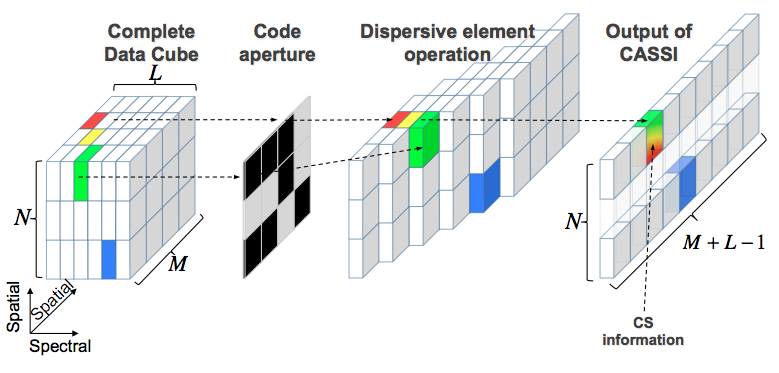
\includegraphics[scale=0.25]{FiguresUpd/cassisensing.png}
\vspace{-10pt}
}
\vspace{-15pt}
\subfigure{
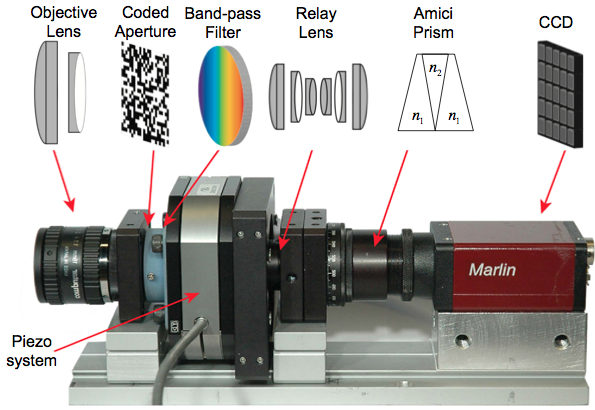
\includegraphics[scale=0.23]{FiguresUpd/cassiarq.png}}
\end{figure}
\footnote{\tiny{A. Wagadarikar, R. John, R. Willett, and D. Brady, “Single disperser design for coded aperture snapshot spectral imaging,” Applied Optics, Vol. 47, No. 10, pp. B44–B51, 2008.}}
\end{frame}

%%%%%%%%%%%%%%%%%%%%%%%%%%%%%

\begin{frame}
\frametitle{Implementation of Coded apertures patterns}

\begin{columns}

\begin{column}{2.5in}
\begin{center}

\textbf{Photomask}\\
\vspace{10pt}
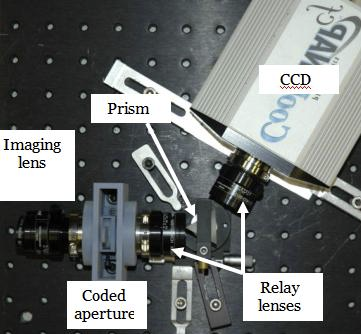
\includegraphics[scale=0.25]{FiguresUpd/photomask.png}
\end{center}

\begin{itemize}
\item \small A new photomask needs to be lithographically fabricated
\item \small The entire system needs to be re-aligned after the installation of the new photomask and it is a very time-consuming process. 
%\item[+] High transmissive efficiency
%\item[--] Low speed and flexibility 
%\item[+] More compact
%\item[+] Pixel size matching
\end{itemize}

\end{column}

\begin{column}{2.5in}
\vspace{-25pt}
\begin{center}
\textbf{Digital Micromirror Device (DMD)}\\
\vspace{10pt}
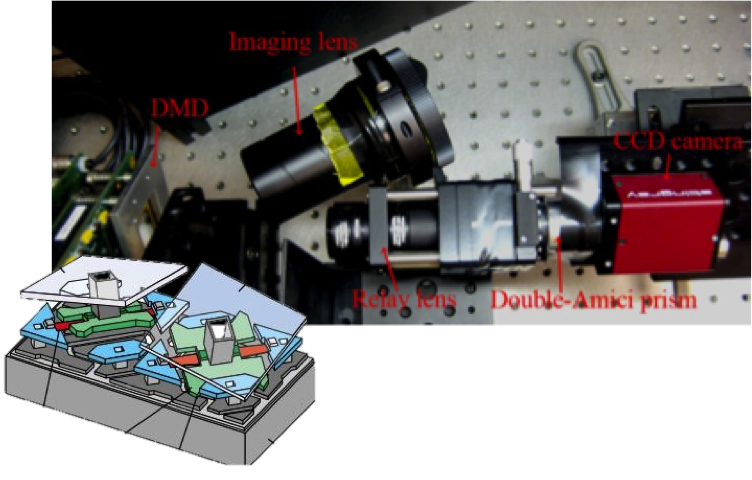
\includegraphics[scale=0.35]{FiguresUpd/dmddmd.png}\\
%\includegraphics[scale=0.33]{figures/dmdcassi3.png}\\
%\vspace{2pt}
%\includegraphics[scale=0.30]{figures/dmdall.png}
\end{center}

\begin{itemize}
\item \small New patterns can be implemented without optical and/or mechanical modification of the system
\item \small Allows multi-shot coding
%\item[--] High reflection efficiency
%\item[+] High sampling speed and Flexibility
%\item[--] Less compact
%\item[--] Pixel size mismatching
\end{itemize}

\end{column}

\end{columns}

\end{frame}

%%%%%%%%%%%%%%%%%%%%%%%%%%%%%

\begin{frame}
\frametitle{Coded Aperture Snapshot Spectral Imager (CASSI)}
\begin{columns}

\begin{column}{3in}
\begin{center}
\includegraphics[scale=0.28]{FiguresUpd/firstmodelb.png}
\end{center}
\end{column}

\begin{column}{2in}
Forward Matrix Model
%\begin{small}
%\begin{equation*}
%\mathbf{g}=\underbrace{\mathbf{H}}_{\text{coding} + \text{dispersion}}\mathbf{f}
%\end{equation*}
\begin{center}
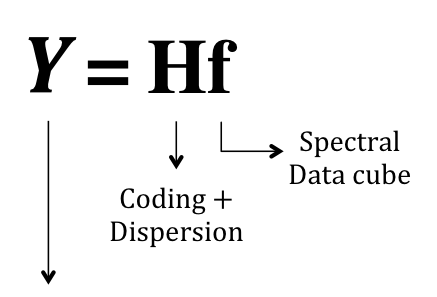
\includegraphics[scale=0.4]{FiguresUpd/Eq3.png}\\
%\vspace{-3pt}
\includegraphics[scale=0.21]{FiguresUpd/measurements.eps}

\end{center}
%\begin{itemize}
%\item $\mathbf{H}$ accounts the coding $\mathbf{T}$ and the dispersion
%\item $\mathbf{f}$ represents the discretized spectral data cube
%\end{itemize}
%\end{small}
\end{column}

\end{columns}

\vspace{-15pt}

\begin{columns}
\begin{column}{1.5in}
\begin{small}
\begin{center}
\vspace{10pt}
Discrete Model
\end{center}
\end{small}
\end{column}

\begin{column}{2.5in}
\vspace{20pt}
\scriptsize
\begin{equation*}
Y_{mn}=\sum_{k=0}^{L-1} \mathcal{F}_{m(n-k)k} T_{m(n-k)}+\omega_{mn}
\end{equation*}
\end{column}
\end{columns}

\end{frame}

%%%%%%%%%%%%%%%%%%%%%%%%%%%%%

%%%%%%%%%%%%%%%%%%%%%%%%%%%%%

%\begin{frame}
%\frametitle{Coded Aperture Snapshot Spectral Imager (CASSI)}
%
%\begin{center}
%\includegraphics[scale=0.30]{figures/firstmodelb.png}
%\end{center}
%
%\vspace{-15pt}
%
%\scriptsize
%\begin{equation*}
%Y_{mn}=\sum_{k=0}^{L-1} \mathcal{F}_{m(n-k)k} T_{m(n-k)}+\omega_{mn}
%\end{equation*}
%
%
%\end{frame}

%%%%%%%%%%%%%%%%%%%%%%%%%%%%%


%\begin{frame}
%\frametitle{Coded Aperture Single Snapshot Imaging (CASSI)}
%\begin{columns}
%\begin{column}{3in}
%\begin{center}
%\includegraphics[scale=0.28]{figures/firstmodel2.png}
%\end{center}
%\end{column}
%\begin{column}{2in}
%Forward Matrix Model
%\begin{small}
%\begin{equation*}
%\mathbf{g=H}\mathbf{f}
%\end{equation*}
%\begin{itemize}
%\item $\mathbf{H}$ accounts the coding $\mathbf{T}$ and the dispersion
%\item $\mathbf{f}$ represents the discretized spectral data cube
%\end{itemize}
%\end{small}
%\end{column}
%\end{columns}
%
%\begin{columns}
%\begin{column}{1.7in}
%\begin{small}
%\begin{center}
%\vspace{-8pt}
%Continuous CASSI Model\\
%\vspace{28pt}
%Discrete Model
%\end{center}
%\end{small}
%\end{column}
%
%\begin{column}{3.2in}
%\scriptsize
%\begin{equation*}
%f_2(x,y,\lambda) = \iint T(x',y')f_0(x',y',\lambda)h(x'-\alpha \lambda - x,y'-y)dx'dy'
%\end{equation*}
%
%
%\scriptsize
%\begin{equation*}
%G_{mn}=\sum_{k=0}^{L-1} \mathcal{F}_{m(n-k)k} T_{m(n-k)+\omega_{mn}}
%\end{equation*}
%\end{column}
%\end{columns}
%
%\end{frame}

%%%%%%%%%%%%%%%%%%%%%%%%%%%%%%

\begin{frame}
\frametitle{Approach: CASSI with Side Information}

\vspace{-10pt}
\begin{figure}
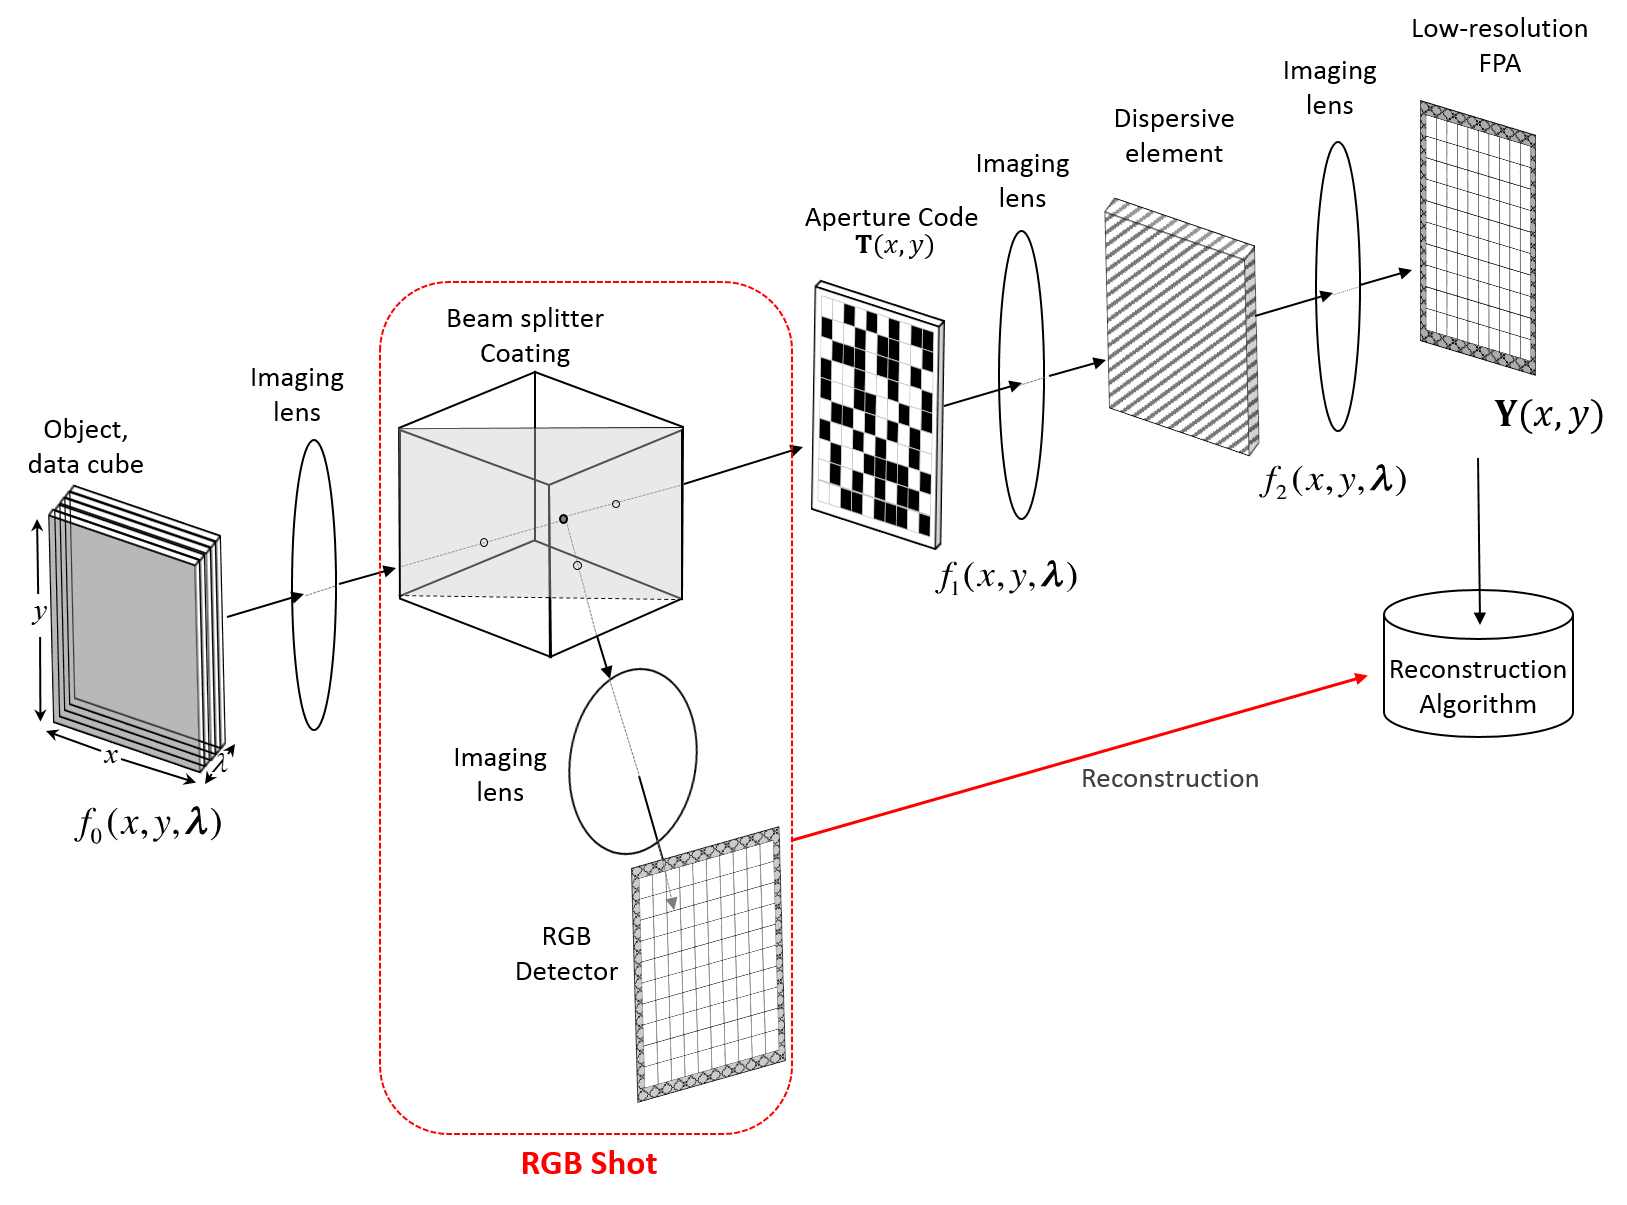
\includegraphics[scale=0.4]{FiguresUpd/systema.png}
\end{figure}

\end{frame}

%%%%%%%%%%%%%%%%%%%%%%%%%%%%%

\begin{frame}
\frametitle{CASSI shot + RGB Side Information}

\vspace{-10pt}
\begin{figure}
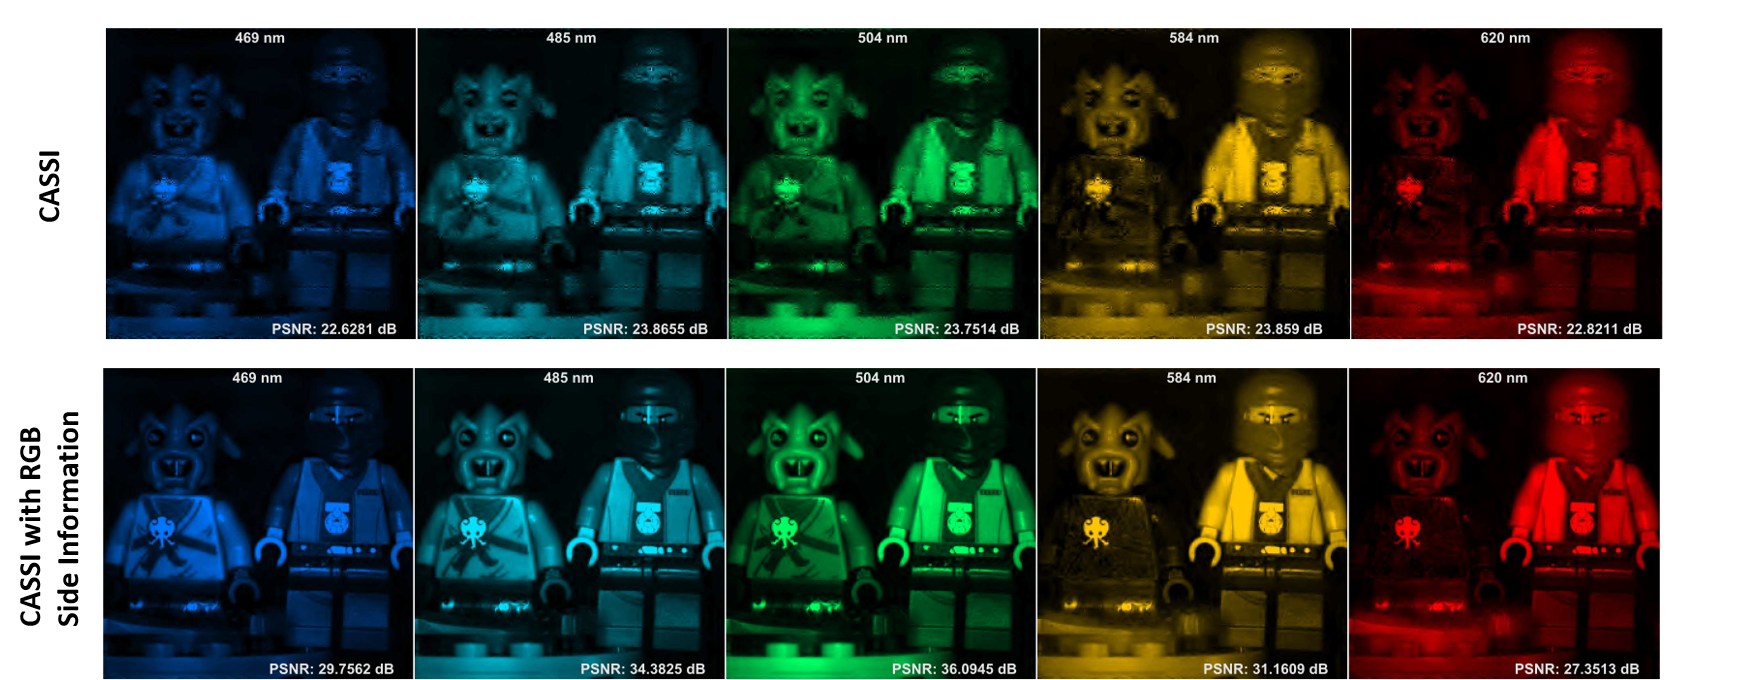
\includegraphics[scale=0.43]{FiguresUpd/CASSIandRGB.png}
\end{figure}

\end{frame}

%%%%%%%%%%%%%%%%%%%%%%%%%%%%%

\begin{frame}
\frametitle{Approach: CASSI with Side Information}

\vspace{-10pt}
\begin{figure}
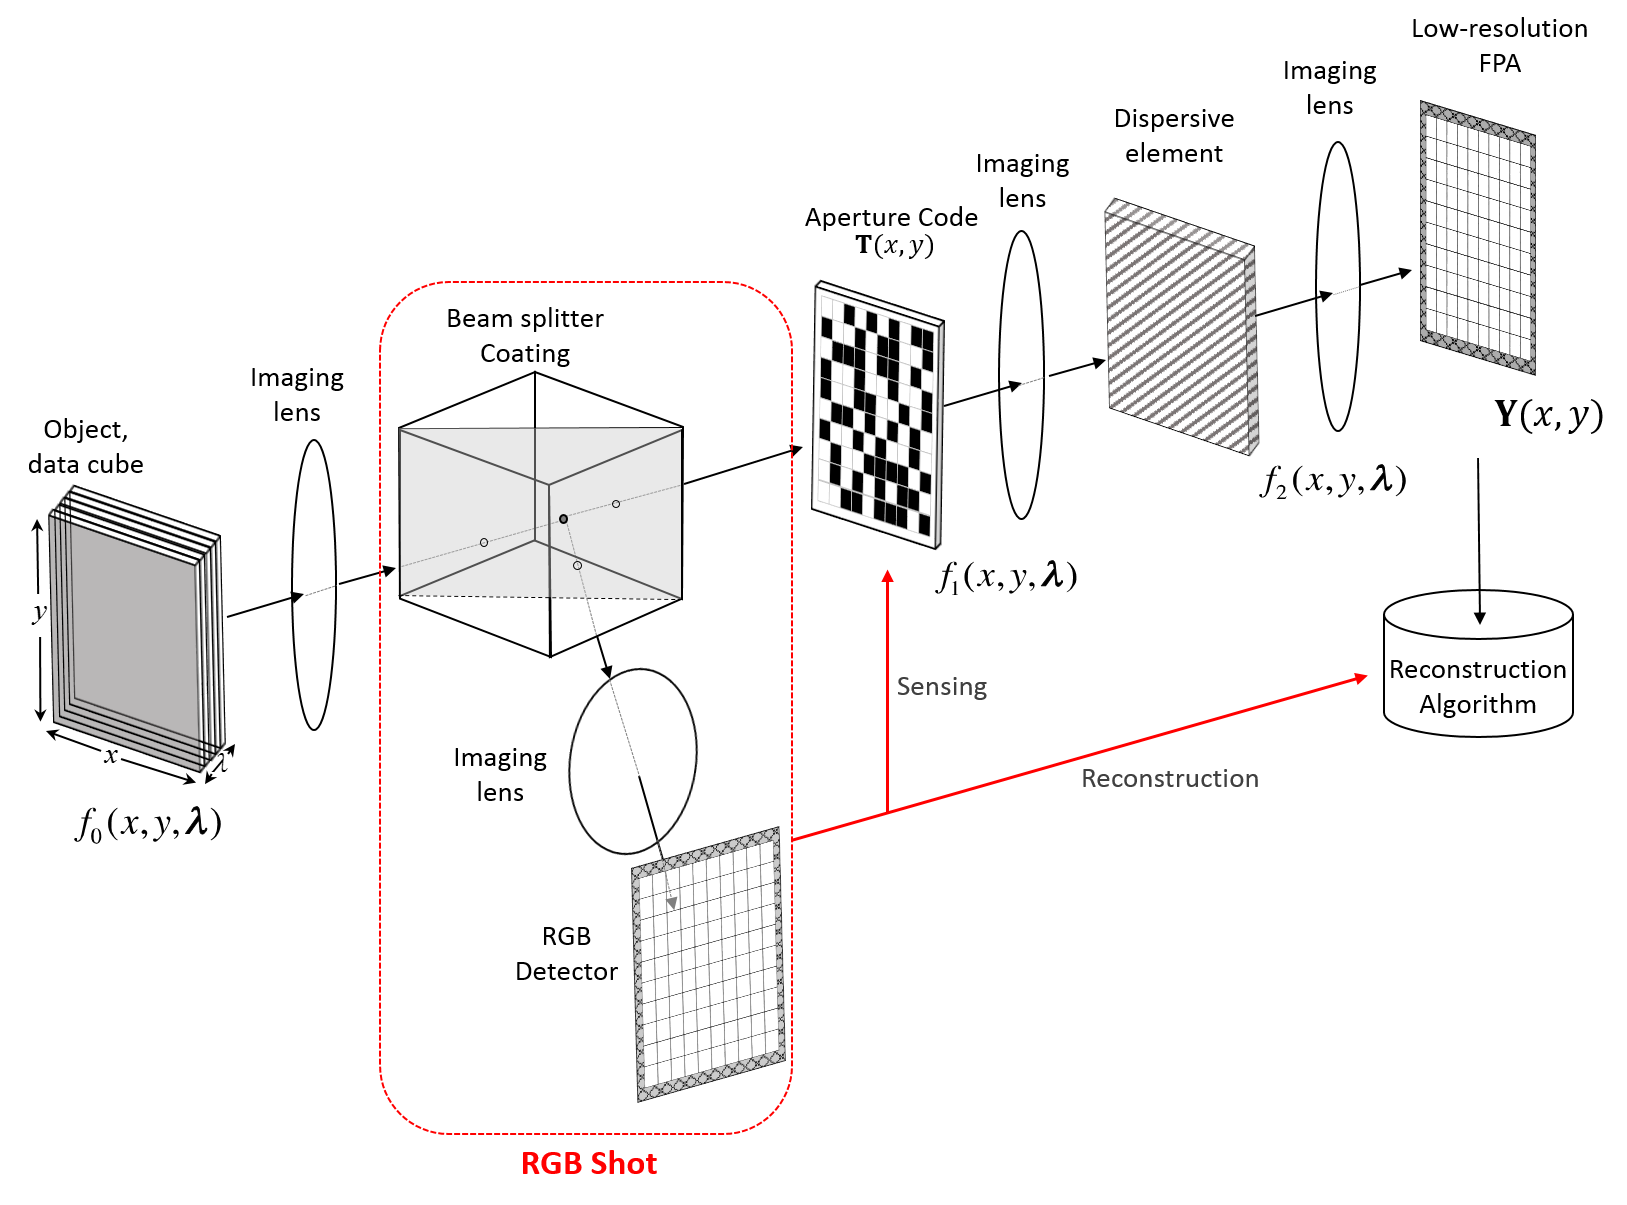
\includegraphics[scale=0.4]{FiguresUpd/system.png}
\end{figure}

\end{frame}

%%%%%%%%%%%%%%%%%%%%%%%%%%%%%

\begin{frame}
\frametitle{Sensing process: Design of coded apertures based on side information}

%\begin{figure}
%\subfigure[Gradient Image $\mathbf{M}$]{\includegraphics[scale=0.42]{figures/real/Borders.png}}
%\subfigure[]{
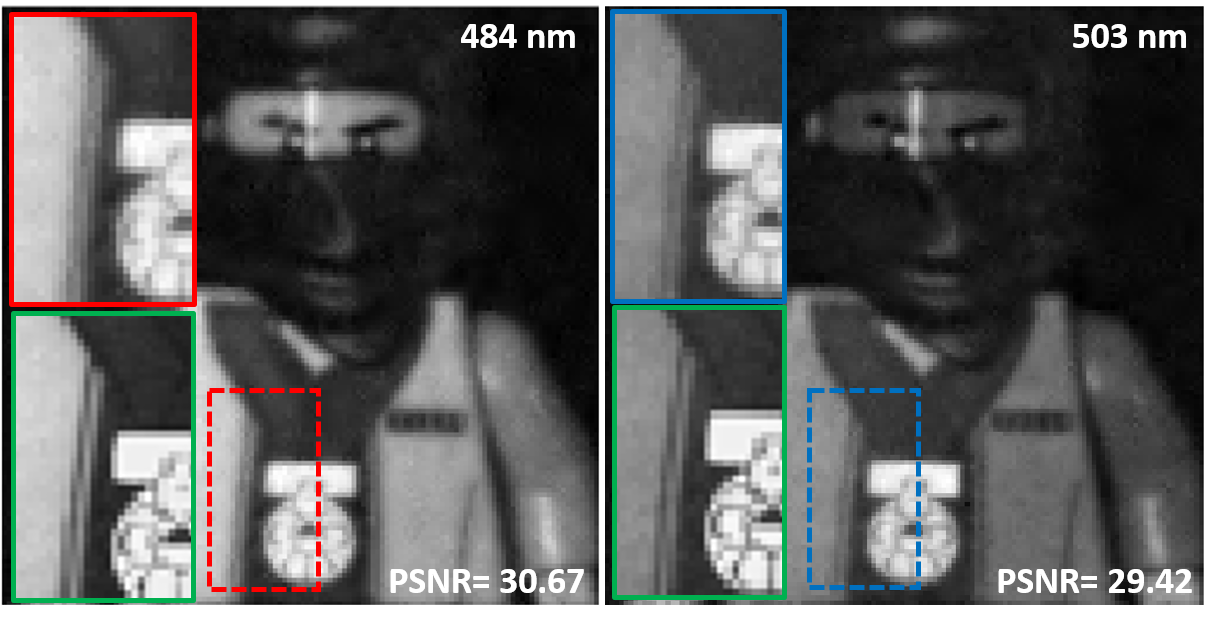
\includegraphics[scale=0.25]{FiguresUpd/Rec.png}
%}
\hspace{20pt}
%\subfigure[]{
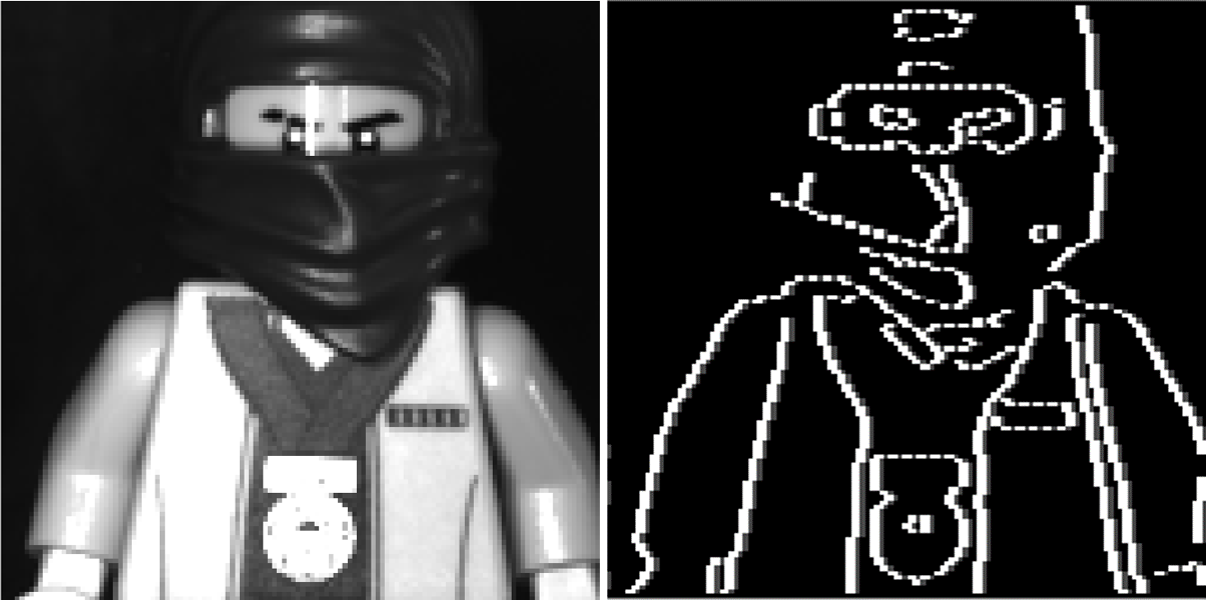
\includegraphics[scale=0.255]{FiguresUpd/Border.png}
%}
\vspace{15pt}
%\subfigure[Correlation between Error reconstruction and borders]{\includegraphics[scale=0.431]{figures/real/Borders_Error.png}}
%\subfigure[]{
\centering
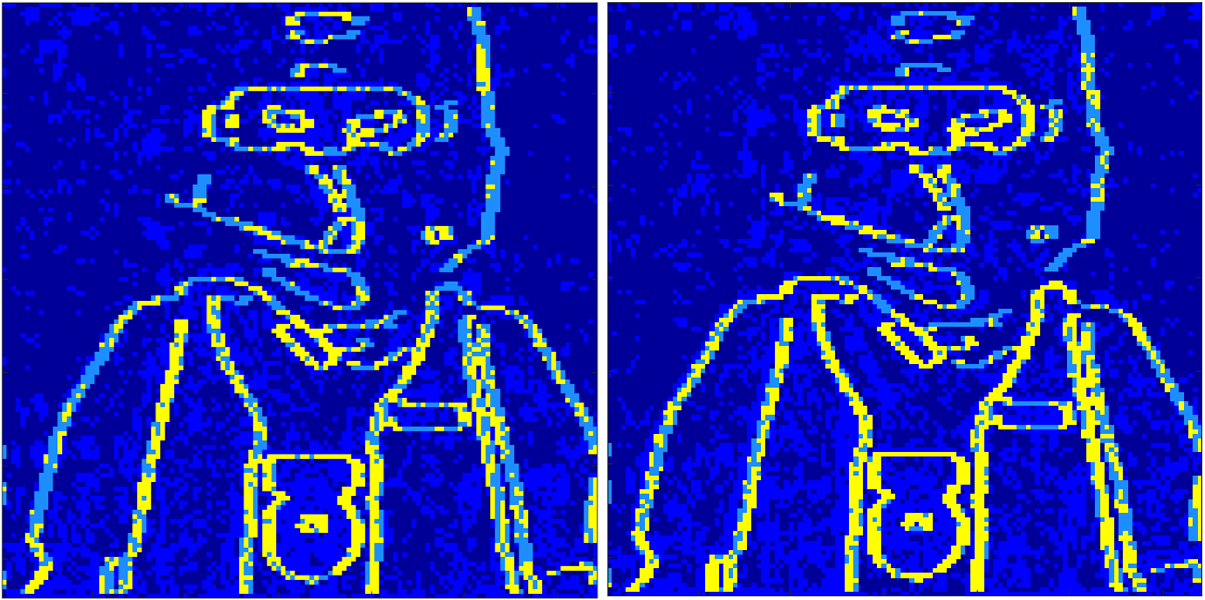
\includegraphics[scale=0.25]{FiguresUpd/Correlation.png}

\footnotesize{Correlation between the reconstruction error and the estimated edges. $19.84\%$ and $14.97\%$ (Yellow pixels) corresponds to errors on the edges.}
%}
%\caption{(a) Two spectral bands reconstructed through simulation of the CASSI system and using a random coded aperture pattern. Zoomed sections are presented in red and blue squares. The original zoomed section is presented in a green square to visually compare the spatial quality of the reconstructions. (b)  Grayscale image of the scene and an estimation of the edges using the Canny method. (c) Correlation between the reconstruction error and the estimated edges in (b) for the two spectral bands in (a).}
%\label{Fig:CorrelationError}
%\end{figure}

\end{frame}

%%%%%%%%%%%%%%%%%%%%%%%%%%%%%%

\begin{frame}
\frametitle{Approach: CASSI with Side Information}


\scriptsize{The $k^{th}$ spectral band of the spatiospectral image:}
\begin{equation*}
\scriptsize
(\mathbf{F}_k)_{mn} \; \Rightarrow \; \mathbf{F}_k=(\mathbf{F}_k)_{mn} \mbox{ for } m,n = 0,\ldots,N-1 \mbox{ and } k=0,1,\ldots,L-1.
\end{equation*}

\scriptsize{Side Information image:}
\begin{equation*}
\scriptsize
\mathbf{F}_G=\sum_{k=0}^{L-1} w_k \mathbf{F}_k \;\;\;\;\; w_k>0,
\label{Eq:Grayscale}
\end{equation*}

\scriptsize{where $\mathbf{w}$ gives the spectral response of the CCD sensor.}

\begin{equation*}
\textcolor{blue}{Canny}(\mathbf{F}_G) = \textcolor{blue}{Canny}\left(\sum_{k=0}^{L-1} w_k \mathbf{F}_k\right).
\label{Eq:GrayscaleEdges1}
\end{equation*}

\scriptsize{The edges of the side information image $\mathbf{F}_G$ are the linear combination of the edges of each band $\mathbf{F}_k$}
\begin{equation*}
\mathbf{\hat{F}}_G = \sum_{k=0}^{L-1} w_k \textcolor{blue}{Canny} \left( \mathbf{F}_k \right) = \sum_{k=0}^{L-1} w_k \mathbf{\hat{F}}_k,
%\label{Eq:GrayscaleEdges2}
\end{equation*}

\scriptsize{Then can be assumed that $\mathbf{\hat{F}}_G$ contains information of all the spectral bands edges, and it is a good estimation of the edges for the spectral bands $\mathbf{\hat{F}}_k$.}

\end{frame}

%%%%%%%%%%%%%%%%%%%%%%%%%%%%%

\begin{frame}

\begin{columns}

\column{2.2in}
\scriptsize{The most representative edges are defined as}
\begin{equation*}
\mathbf{\left( \overline{F}_G\right) }_{mn} = 
\begin{cases} 
\left( \mathbf{\hat{F}}_{G} \right)_{mn}, & \mbox{if } \left( \mathbf{\hat{F}}_G \right)_{mn} > \rho \\ 
0, & \mbox{otherwise},
\end{cases}
\label{Eq:Fg}
\end{equation*}

\textbf{\scriptsize{Design of the codes}}

\begin{equation*}
\mathbf{T} = \mathbf{T}_{b1} \cdot \mathbf{T}_e + \mathbf{T}_{b2} \cdot (1-\mathbf{T}_e),
\label{Eq:T1}
\end{equation*}

\begin{equation*}
\mathbf{T} = \mathbf{T}_{b1} \cdot \mathbf{\overline{F}}_G + \mathbf{T}_{b2} \cdot (1-\mathbf{\overline{F}}_G).
\end{equation*}

\begin{itemize}
\item First component: Blue noise pattern (in order to achieve a more uniform sensing)
\item Second component: Edge component
\item $\mathbf{T}_{b1}\neq \mathbf{T}_{b2}$
\end{itemize}

\column{3in}
\begin{figure}
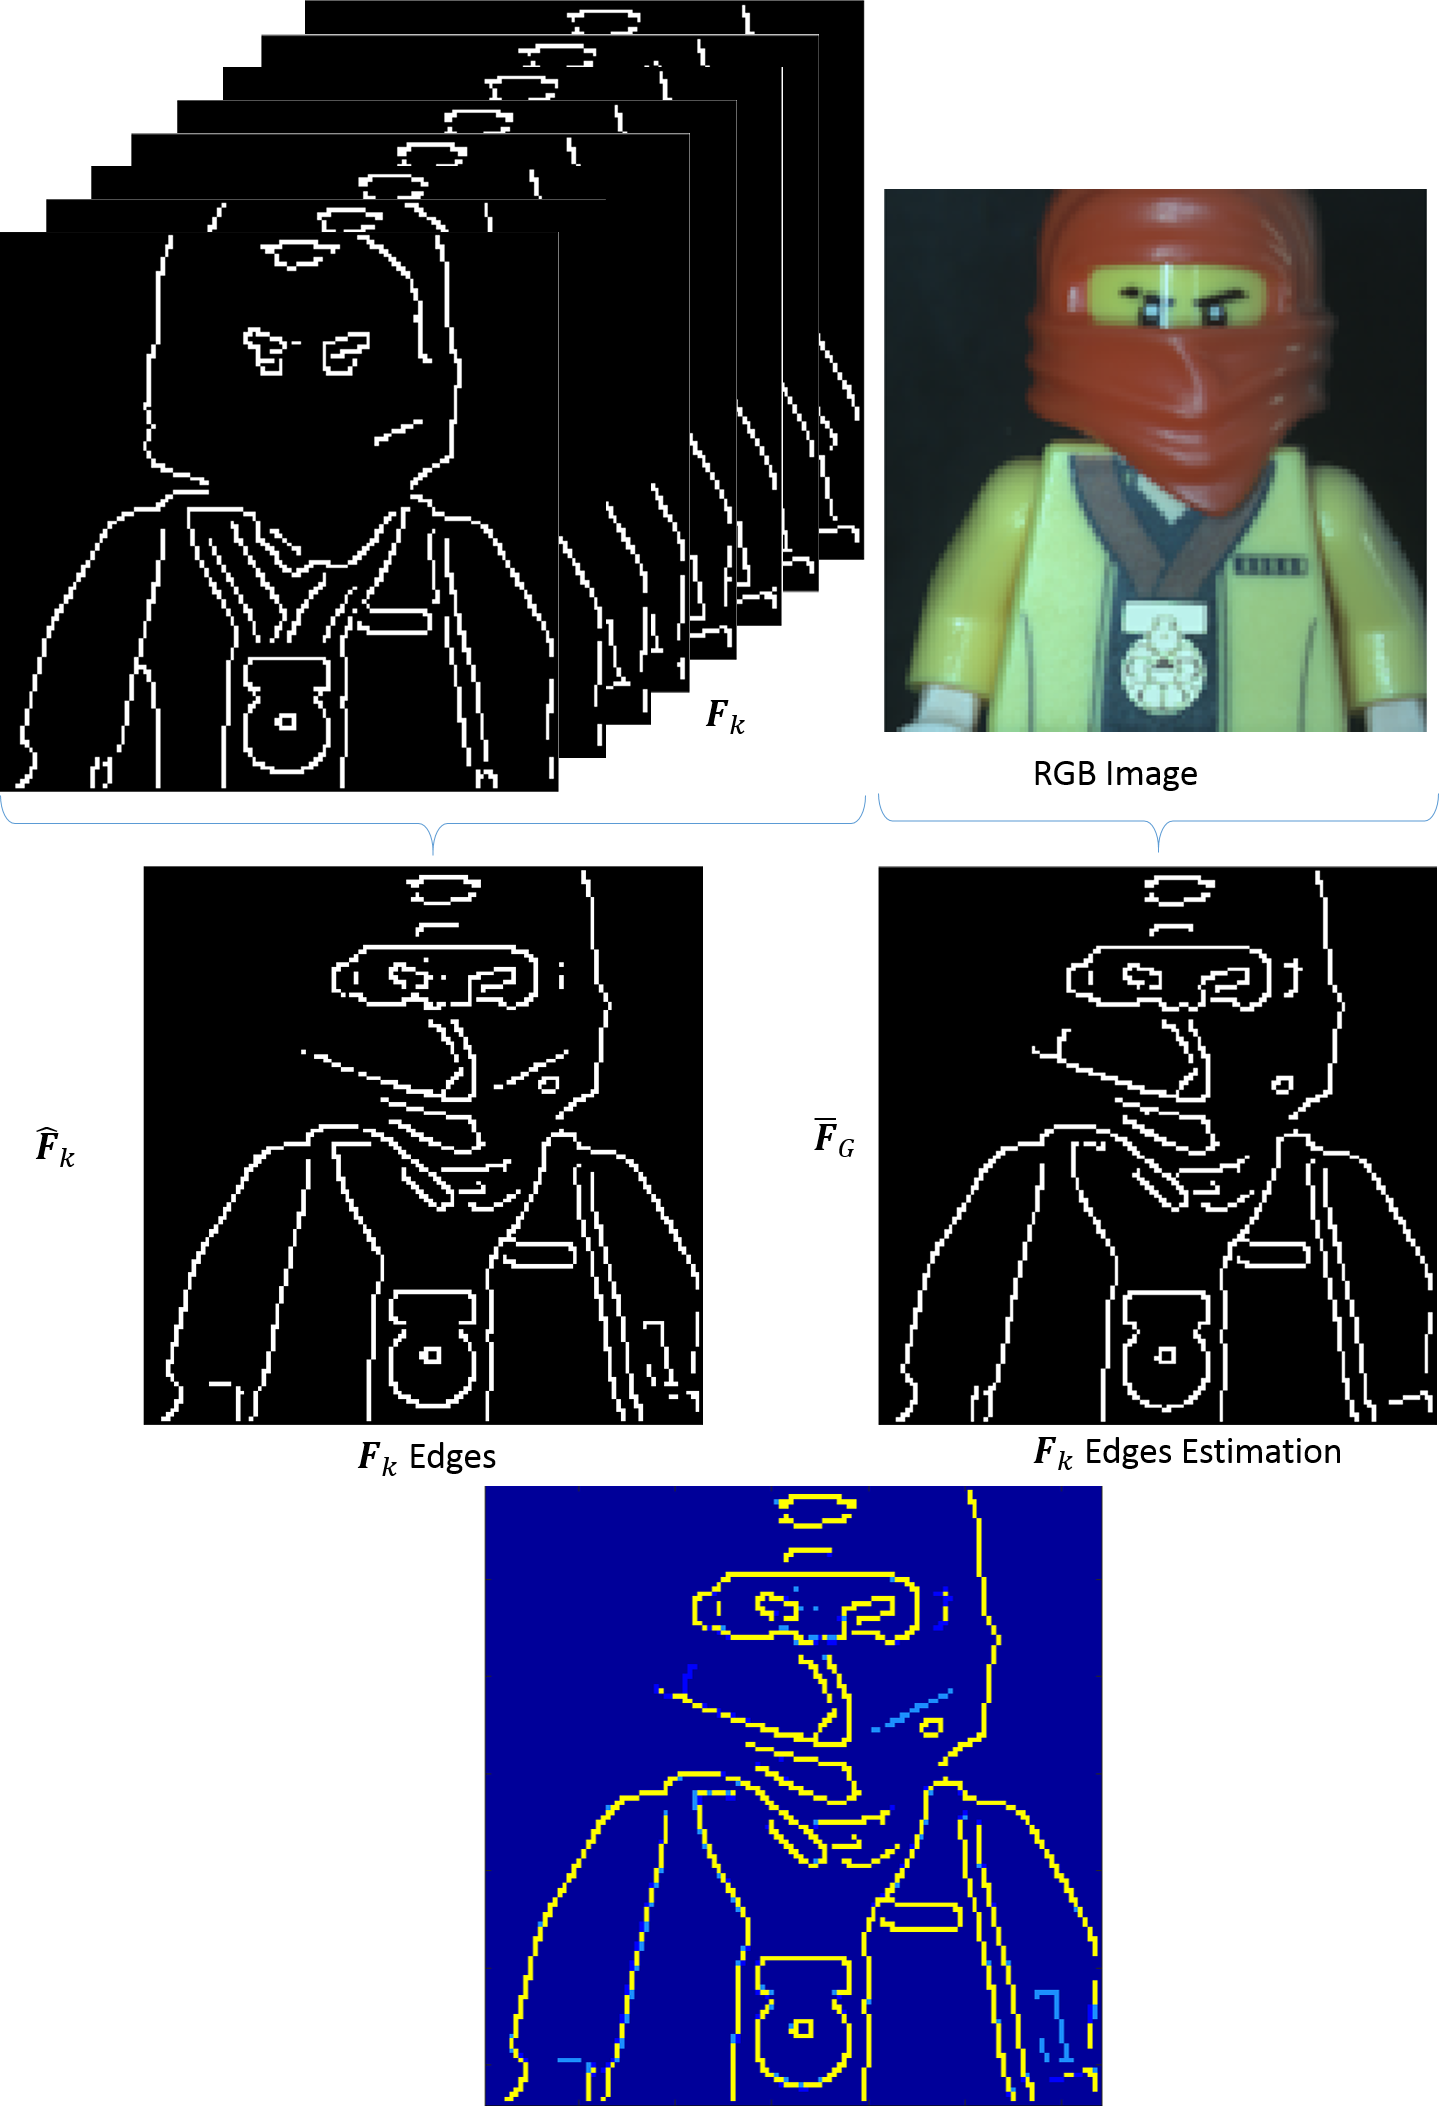
\includegraphics[scale=0.22]{FiguresUpd/edgesestimation.png}
\end{figure}

\end{columns}
 
\end{frame}

%%%%%%%%%%%%%%%%%%%%%%%%%%%%%

\begin{frame}
\frametitle{Approach: CASSI with Side Information}

\vspace{-15pt}
\begin{equation*}
\small
Y_{mn} \!\! = \!\!\! \sum_{k=0}^{L-1}  \left[  \left( \mathbf{T}_{b1} \right)_{m(n-k)} \!\! \left( \mathbf{\overline{F}}_G \right)_{m(n-k)} \!\! + \!  \left( \mathbf{T}_{b2} \right)_{m(n-k)} \!\! \left(1- \mathbf{\overline{F}}_G \right)_{m(n-k)} \right]  \left( \mathbf{F}_k  \right)_{m(n-k)}
\end{equation*}

%\begin{equation*}
%\mathbf{\left( \hat{\overline{F}}_k\right) }_{mn} = 
%\begin{cases} 
%\mathbf{\left( F_{k} \right) }_{mn}, & \mbox{if } \left( \mathbf{\overline{F}}_G \right)_{mn} > \eta \\ 
%0, & \mbox{otherwise}
%\end{cases}
%\label{Eq:Fgfinal}
%\end{equation*}

\begin{block}{}
\begin{equation*}
\begin{scriptsize}
Y_{mn} \! = \underbrace{ \! \sum_{k=0}^{L-1} \! (\mathbf{T}_{b1})_{m(n-k)} \!\! \left( \mathbf{\overline{F}}_k \right)_{m(n-k)} \left( \mathbf{F}_k  \right)_{m(n-k)}  }_{\mbox{a. Sensing of edge sections}} + \underbrace{\! \sum_{k=0}^{L-1} \!\! \left( \mathbf{T}_{b2} \right)_{m(n-k)} \!\! \left(1- \mathbf{\overline{F}}_G \right)_{m(n-k)} \!\! \left( \mathbf{F}_k  \right)_{m(n-k)}}_{\mbox{b. Sensing of background}},
\end{scriptsize}
\end{equation*}
\end{block}

\vspace{-10pt}

\begin{itemize}
\item \scriptsize{Several coded apertures patterns can be calculated}
\item \scriptsize{Transmittance of the final coded aperture is in the range of $16\% - 26\%$}
\item \scriptsize{The width of the edges give us many more options of coded apertures to test}
\item $\mathbf{T}_{b1}\neq \mathbf{T}_{b2}$
\item It is possible to use low or high transmittances in the borders
\end{itemize}

\end{frame}



%%%%%%%%%%%%%%%%%%%%%%%%%%%%%

\begin{frame}
\frametitle{Reconstruction Process}


\begin{columns}
\column{2in}

Optimization Problem

\begin{equation*}
\small
\tilde{\mathbf{f}} = \pmb{\Psi}\lbrace\text{argmin}_{\pmb{\theta}}\vert\vert \mathbf{y}-\mathbf{H}\pmb{\Psi}\pmb{\theta}\vert\vert_2+\tau \vert\vert \pmb{\theta}\vert\vert_1\rbrace
\end{equation*}

\begin{itemize}%[leftmargin=*]
\item $\pmb{\theta}$ is an $S$-sparse representation of $\mathbf{f}$
\item $\tau$ is a regularization constant
\item $\pmb{\Psi}=\pmb{\Psi}_1 \bigotimes \pmb{\Psi}_2$, 
\begin{itemize}
\item $\pmb{\Psi}_1$ is a 2D-Wavelet Symmlet 8 basis 
\item $\pmb{\Psi}_2$ is the 1D-Discrete Cosine Transform
\end{itemize}

\item GPSR algorithm is used to obtain the reconstructions
\end{itemize}

\column{2.5in}
\begin{figure}
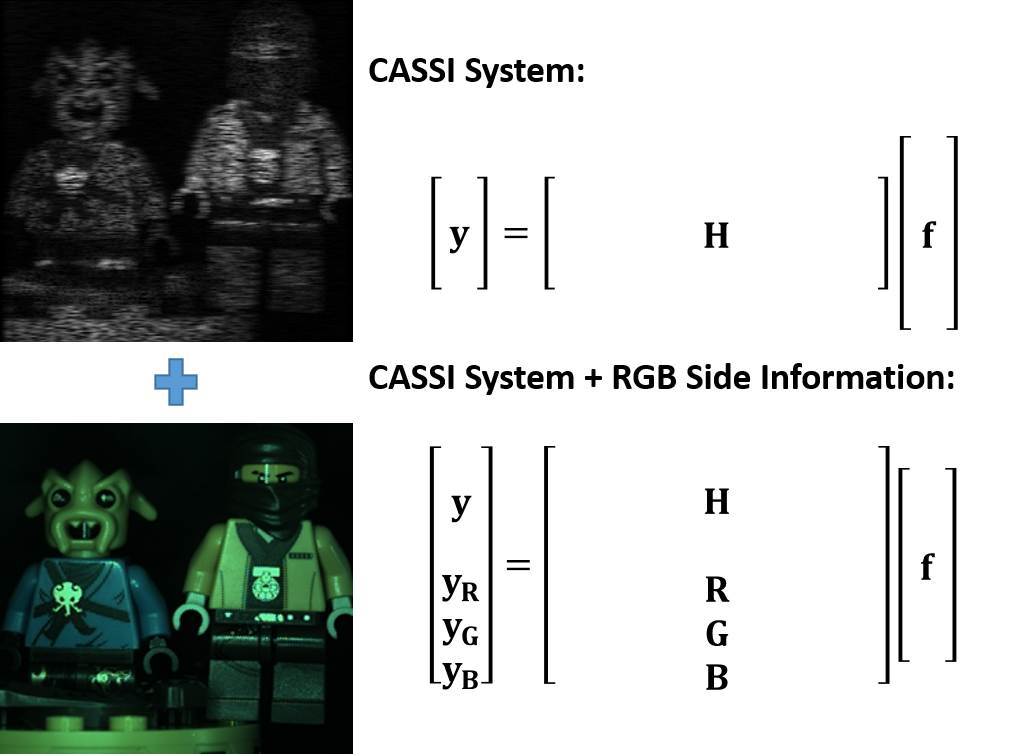
\includegraphics[scale=0.35]{FiguresUpd/CASSIandRGBrec.png}
\end{figure}

\vspace{-20pt}

\begin{figure}
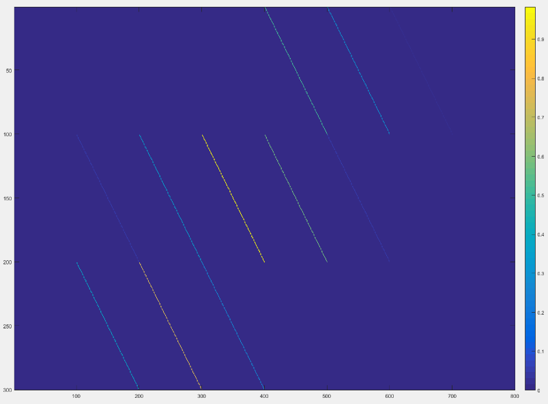
\includegraphics[scale=0.4]{FiguresUpd/HRGB.png}
\end{figure}
\end{columns}

\end{frame}

%%%%%%%%%%%%%%%%%%%%%%%%%%%%%

%%%%%%%%%%%%%%%%%%%%%%%%%%%%%%

%\begin{frame}
%\frametitle{Example: Synthetic coded aperture}
%
%\begin{figure}
%\includegraphics[scale=0.4]{figures/codetransformation33.png}
%\end{figure}
%\end{frame}

%%%%%%%%%%%%%%%%%%%%%%%%%%%%%

\section{Simulations results}
\begin{frame}
\frametitle{Simulations results}

\begin{columns}
\column{3.5in}
\begin{itemize}
\item Test data cube $\mathcal{F}$: $128 \times 128 \times 8$ 
\item Reconstruction algorithm: GPSR
\item Designed coded aperture $T= 0.23$
\item Random coded aperture $T= 0.25 - 0.5$
\end{itemize}

\column{2in}
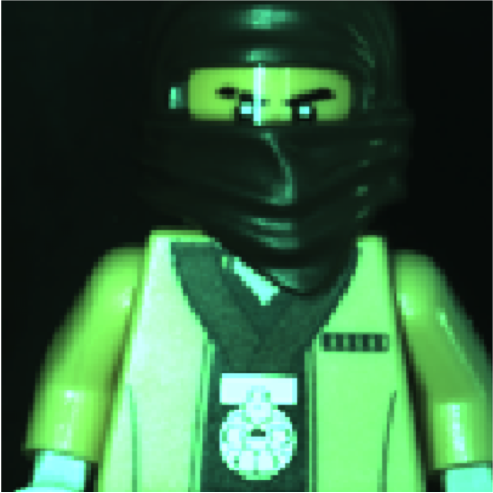
\includegraphics[scale=0.38]{FiguresUpd/sim_rgb.png}

\end{columns}

\begin{figure}
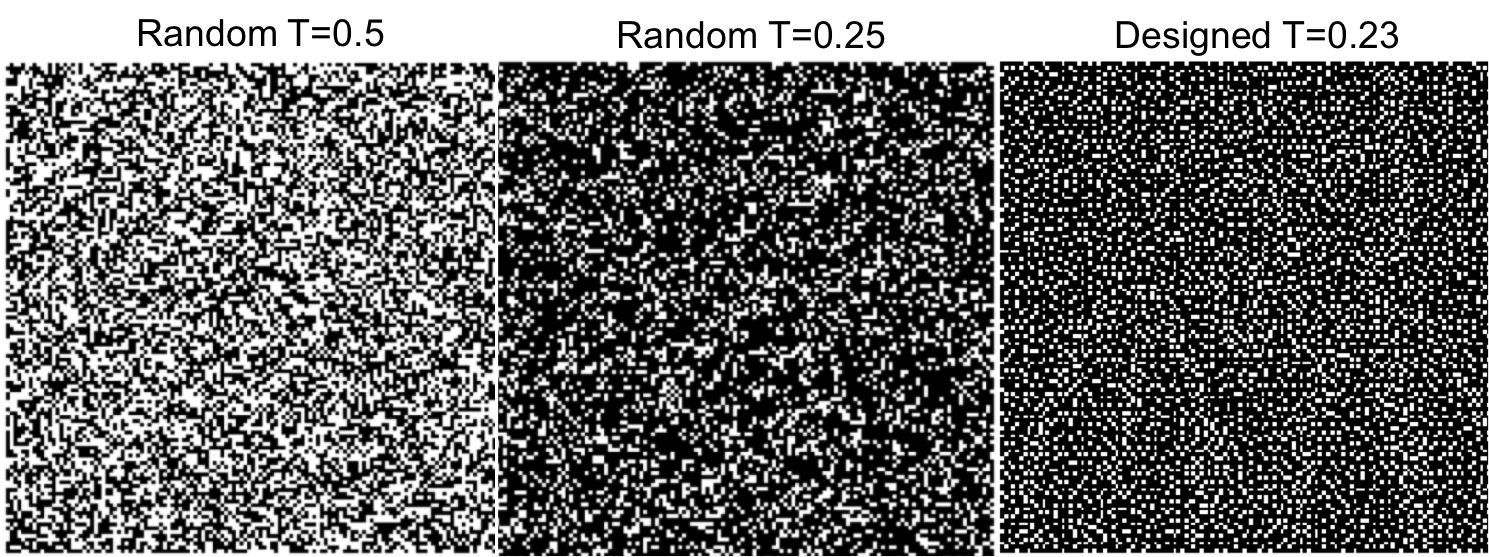
\includegraphics[scale=0.4]{FiguresUpd/codes.png}
\end{figure}
\end{frame}

%%%%%%%%%%%%%%%%%%%%%%%%%%%%%

\begin{frame}

\begin{figure}
\centering
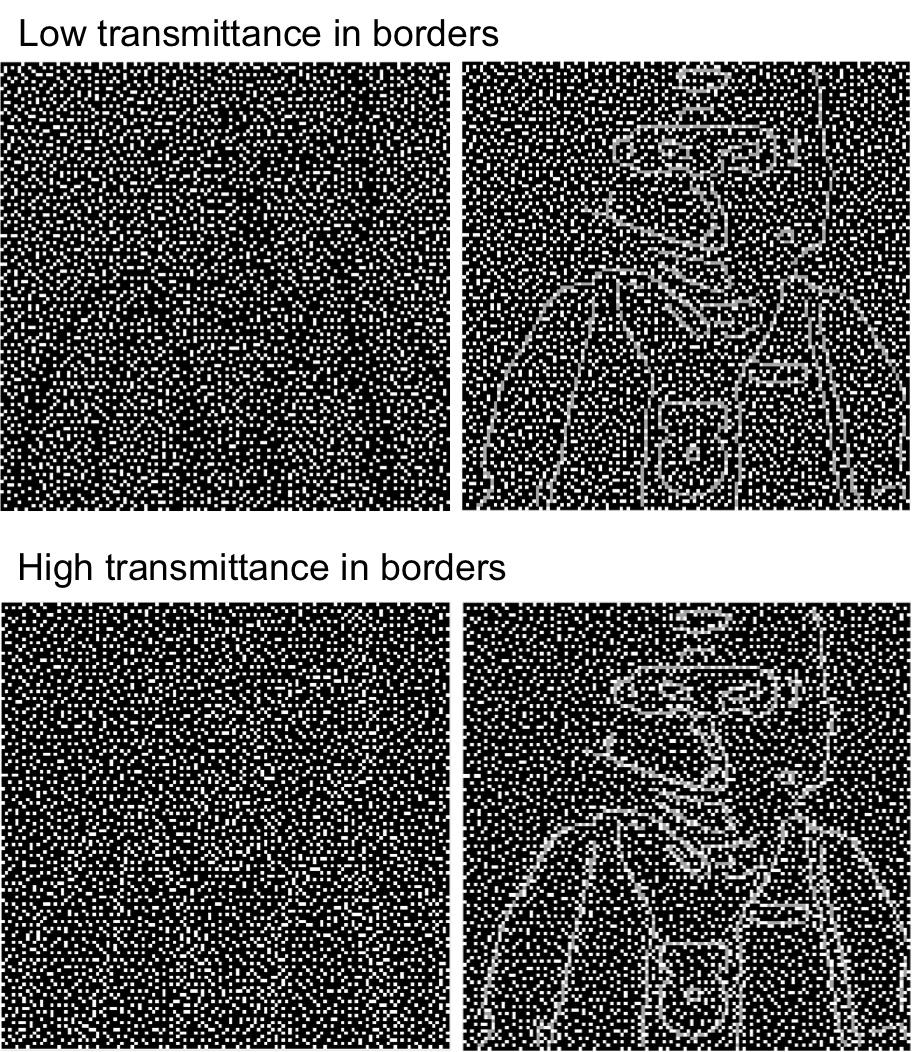
\includegraphics[scale=0.5]{FiguresUpd/bordersCode.png}
\end{figure}
\end{frame}

%%%%%%%%%%%%%%%%%%%%%%%%%%%%%

\begin{frame}
\frametitle{Random coded apertures $T=0.25$}

\begin{figure}
\centering
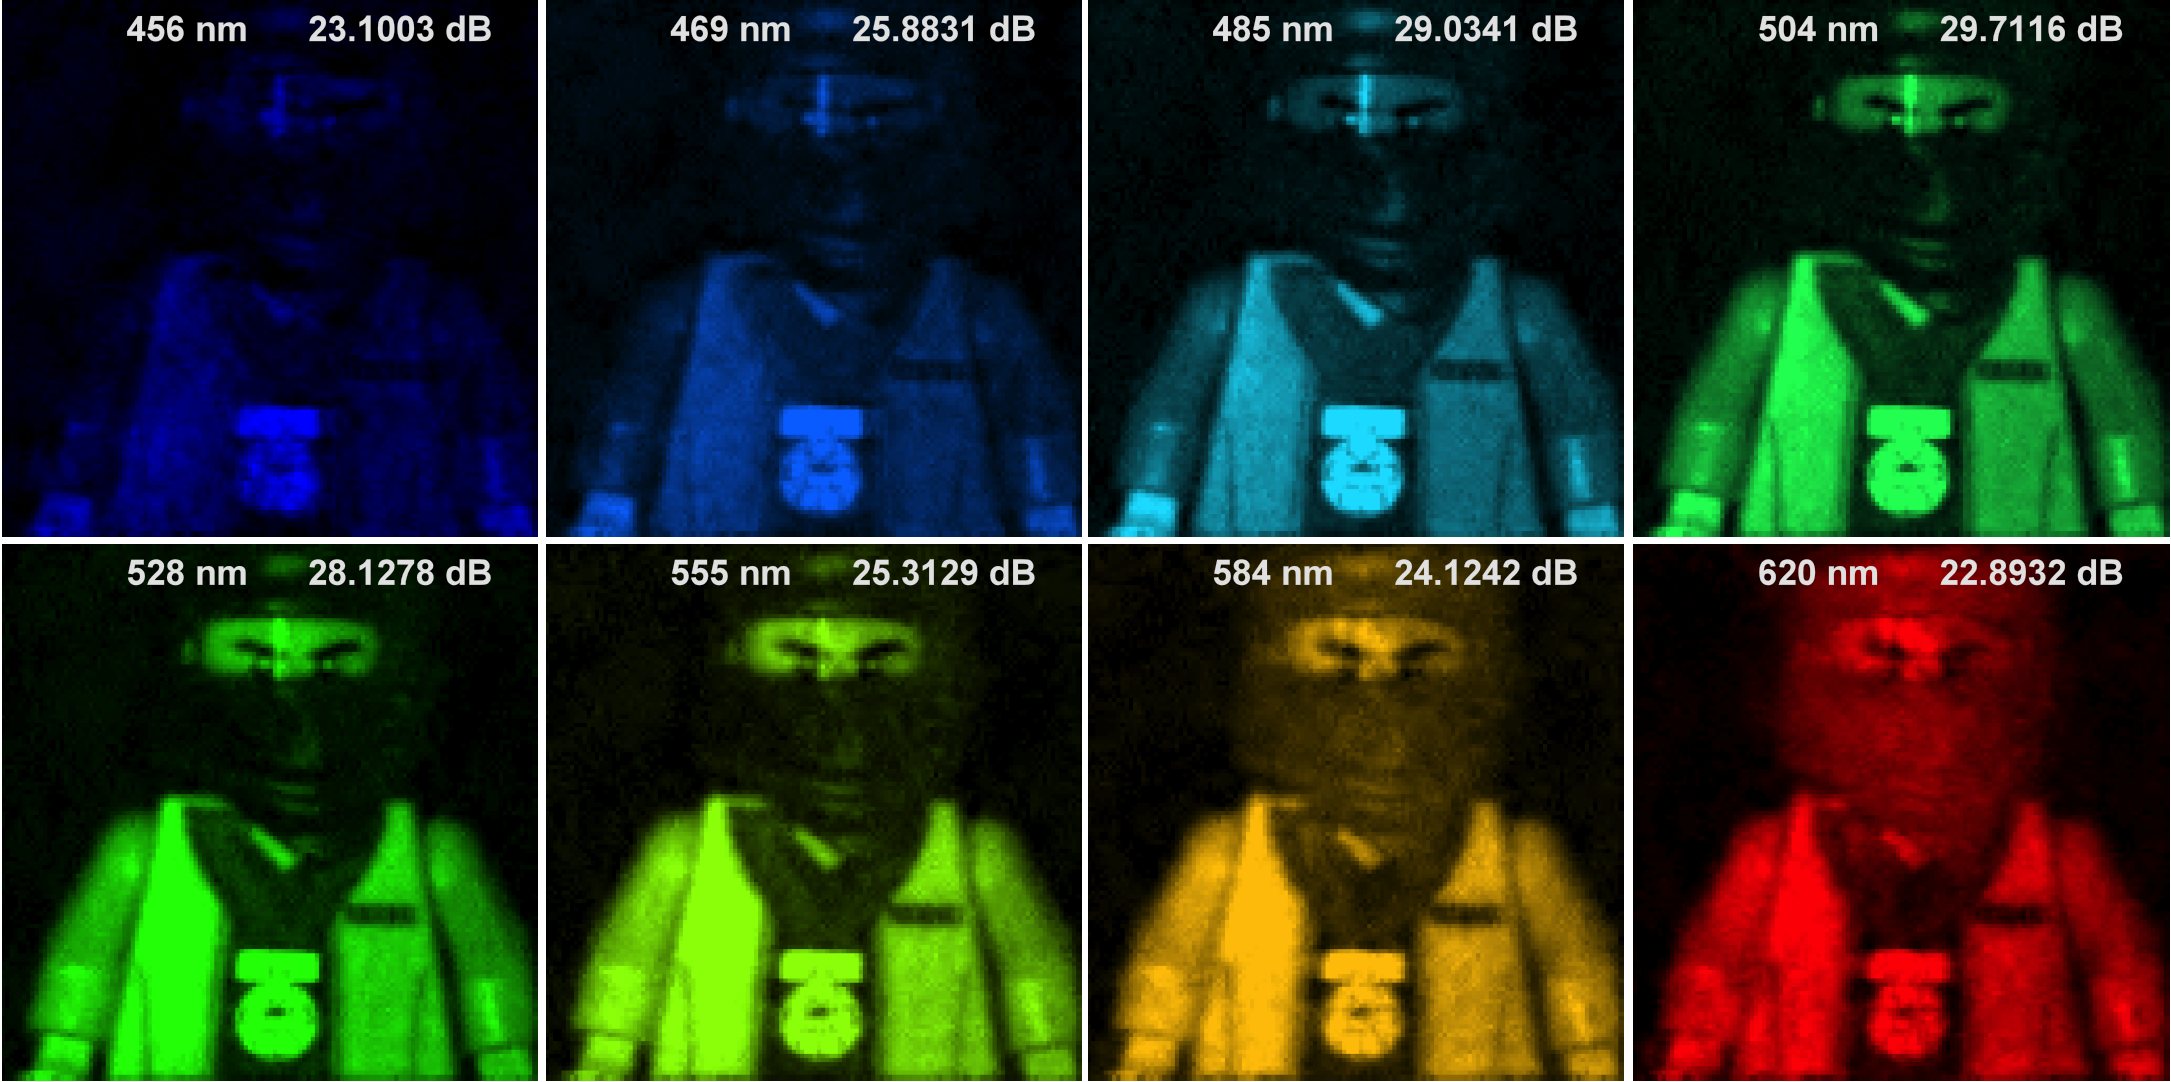
\includegraphics[scale=0.30]{FiguresUpd/Sim_rand025.png}
\end{figure}
%\begin{scriptsize}
%(Left) Original data cube mapped to a RGB profile. (Center) Reconstruction using CASSI and (right), reconstruction using the CASSI with synthetic coded apertures model.
%\end{scriptsize}
\end{frame}

%%%%%%%%%%%%%%%%%%%%%%%%%%%%%

\begin{frame}
\frametitle{Designed coded apertures $T=0.23$}

\begin{figure}
\centering
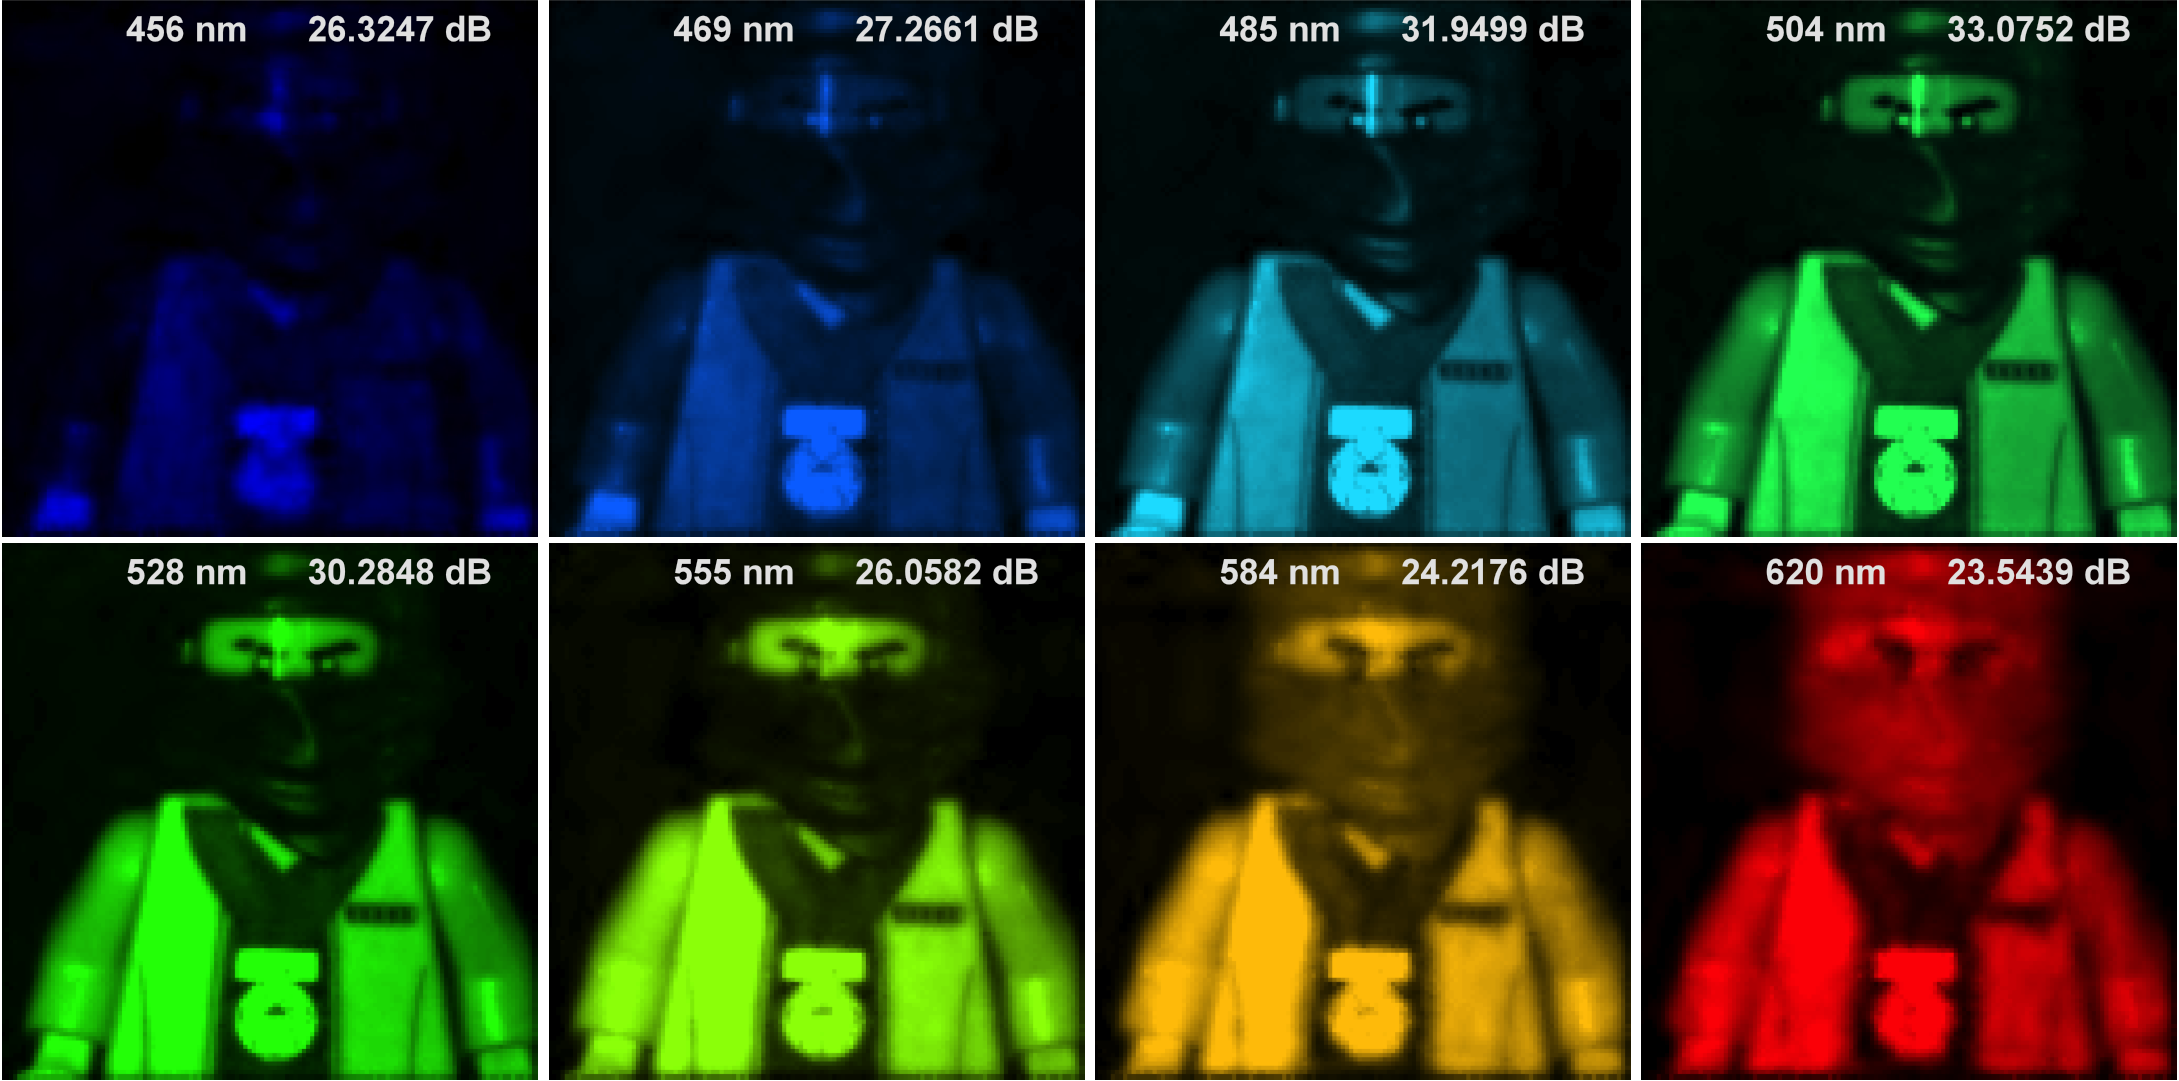
\includegraphics[scale=0.30]{FiguresUpd/Sim_desig023.png}
\end{figure}
%\begin{scriptsize}
%(Left) Original data cube mapped to a RGB profile. (Center) Reconstruction using CASSI and (right), reconstruction using the CASSI with synthetic coded apertures model.
%\end{scriptsize}
\end{frame}

%%%%%%%%%%%%%%%%%%%%%%%%%%%%%

\begin{frame}
\frametitle{Random coded apertures $T=0.5$}

\begin{figure}
\centering
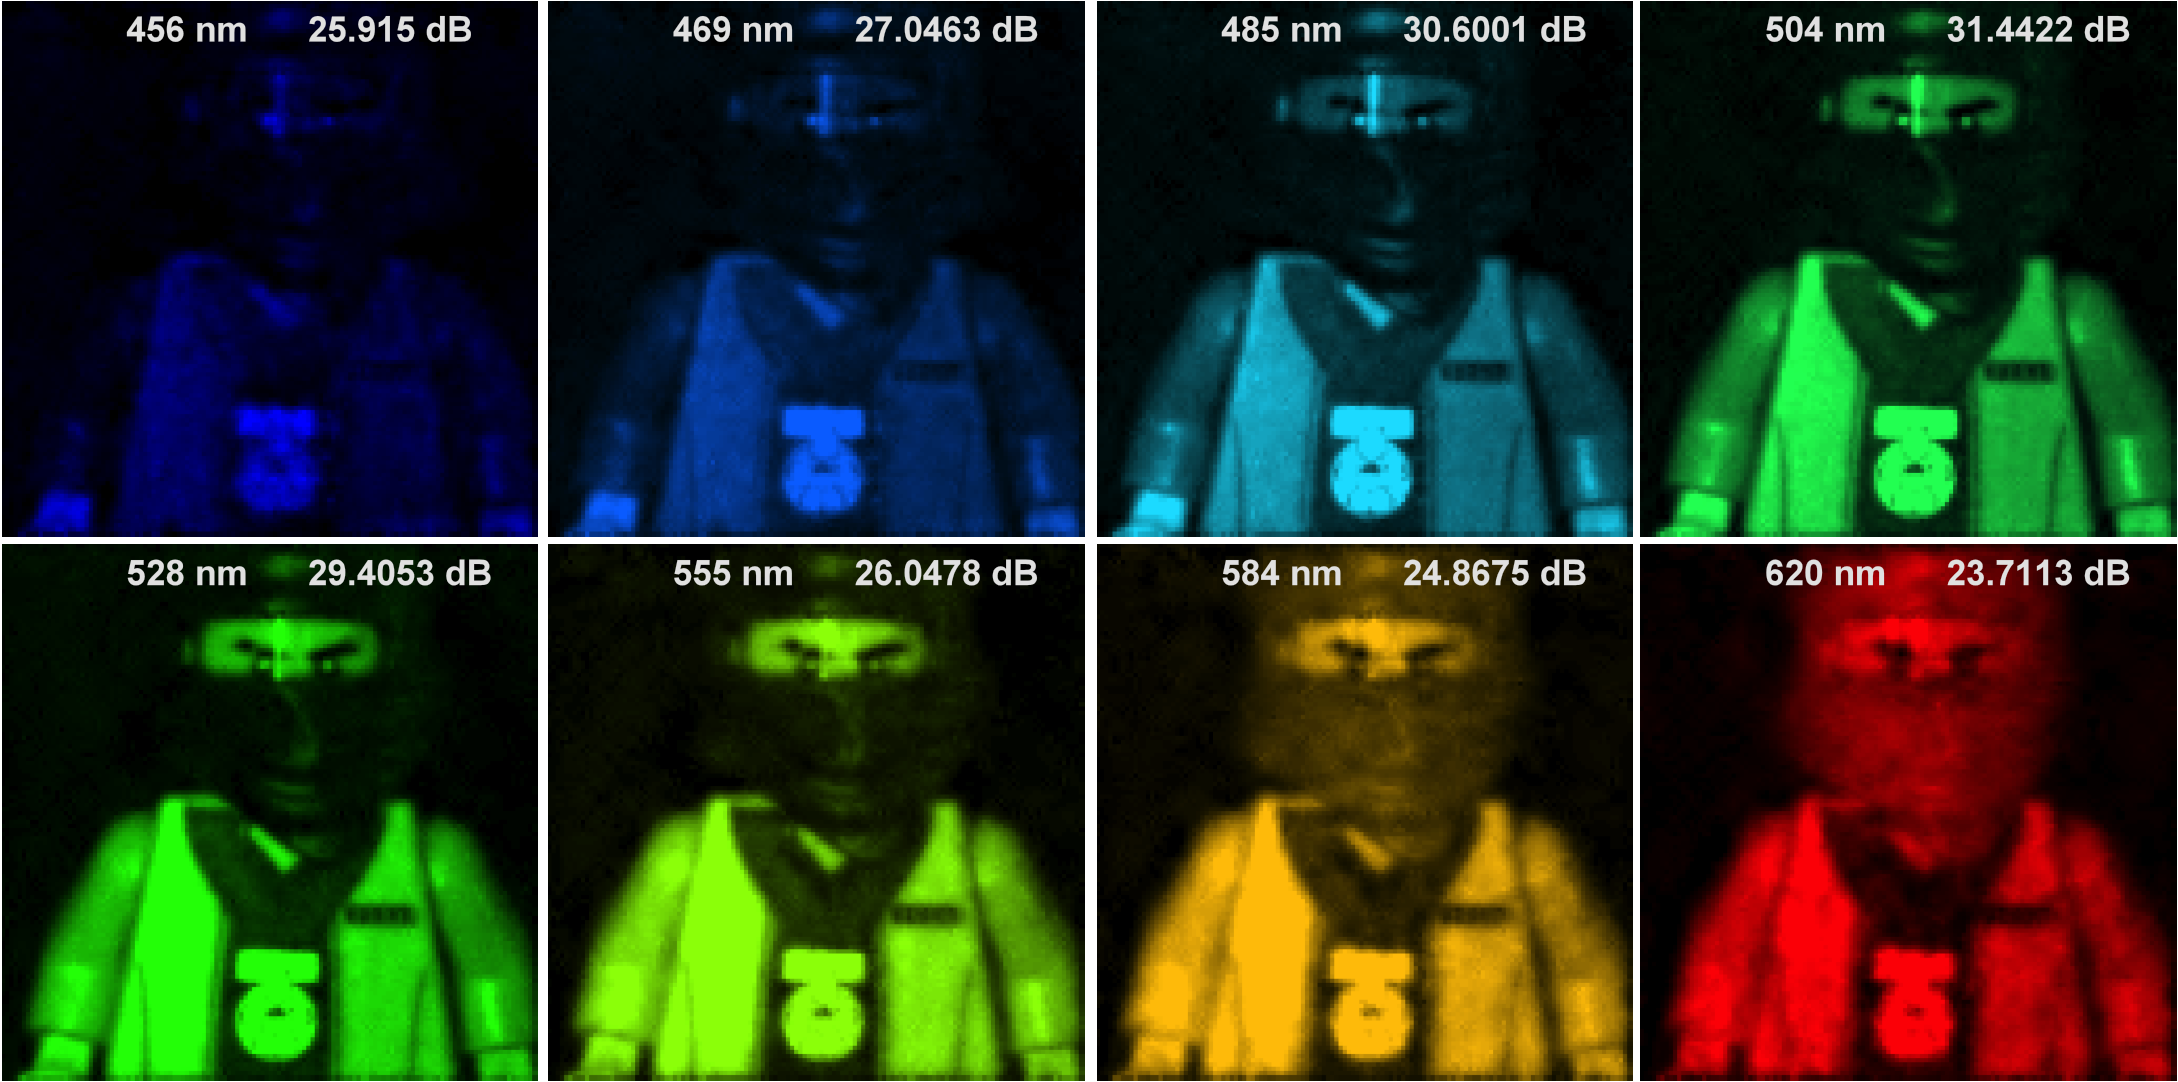
\includegraphics[scale=0.30]{FiguresUpd/Sim_rand05.png}
\end{figure}
%\begin{scriptsize}
%(Left) Original data cube mapped to a RGB profile. (Center) Reconstruction using CASSI and (right), reconstruction using the CASSI with synthetic coded apertures model.
%\end{scriptsize}
\end{frame}

%%%%%%%%%%%%%%%%%%%%%%%%%%%%%

\begin{frame}

\begin{figure}
\centering
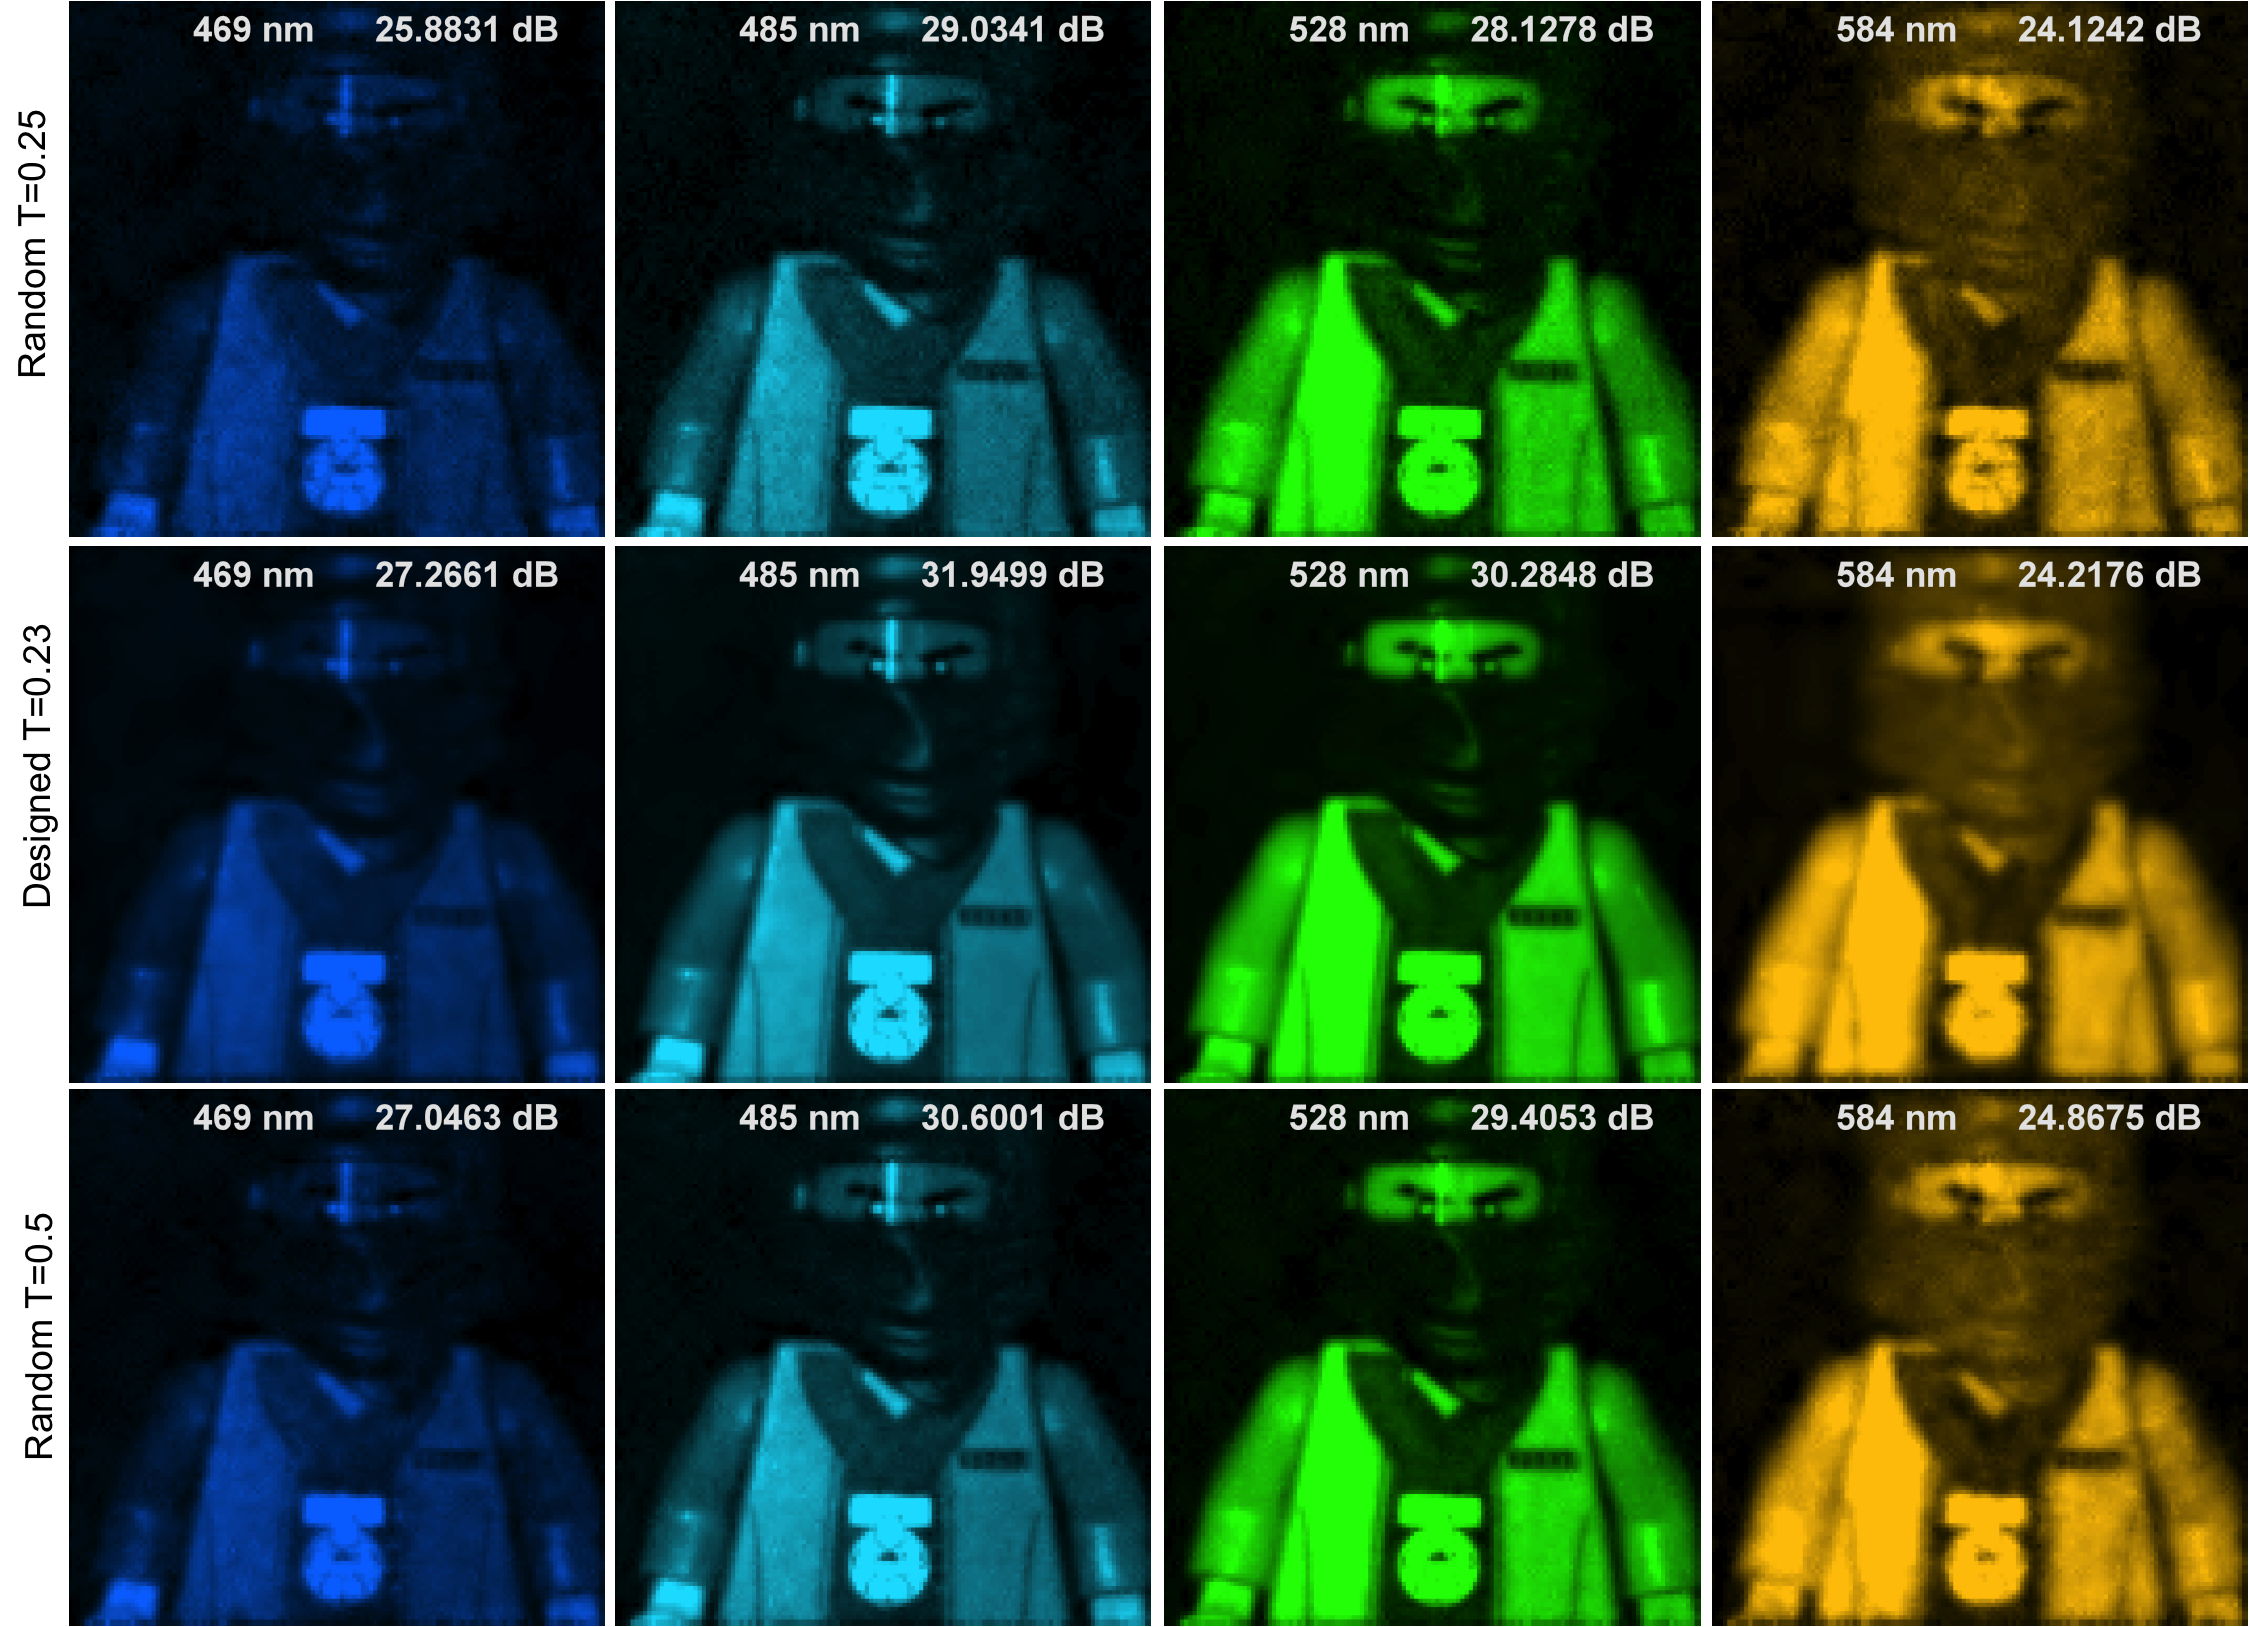
\includegraphics[scale=0.3]{FiguresUpd/Sim_all.png}
\end{figure}
%\begin{scriptsize}
%(Left) Original data cube mapped to a RGB profile. (Center) Reconstruction using CASSI and (right), reconstruction using the CASSI with synthetic coded apertures model.
%\end{scriptsize}
\end{frame}

%%%%%%%%%%%%%%%%%%%%%%%%%%%%%

\begin{frame}
\frametitle{Spectral Reconstruction}

\begin{figure}
\centering
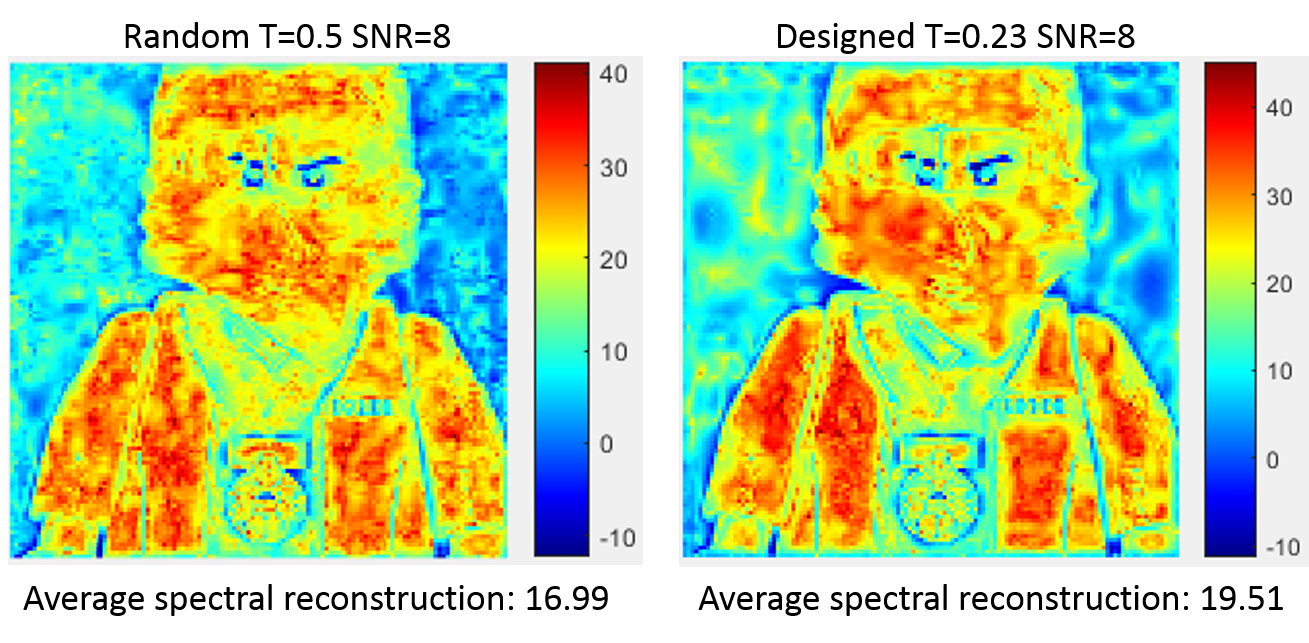
\includegraphics[scale=0.5]{FiguresUpd/spectral.png}
\end{figure}
%\begin{scriptsize}
%(Left) Original data cube mapped to a RGB profile. (Center) Reconstruction using CASSI and (right), reconstruction using the CASSI with synthetic coded apertures model.
%\end{scriptsize}
\end{frame}

%%%%%%%%%%%%%%%%%%%%%%%%%%%%%

\begin{frame}
\frametitle{SNR analysis}

\begin{figure}
\centering
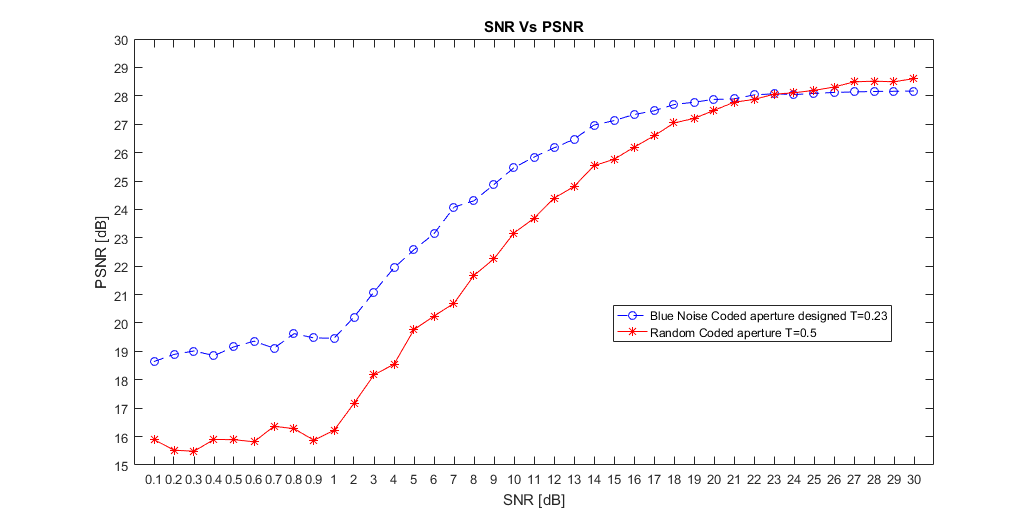
\includegraphics[scale=0.45]{FiguresUpd/SNRvsPSNR.png}
\end{figure}
\end{frame}

%%%%%%%%%%%%%%%%%%%%%%%%%%%%%


\begin{frame}
\frametitle{Selection of coded apertures}

\begin{figure}
\centering
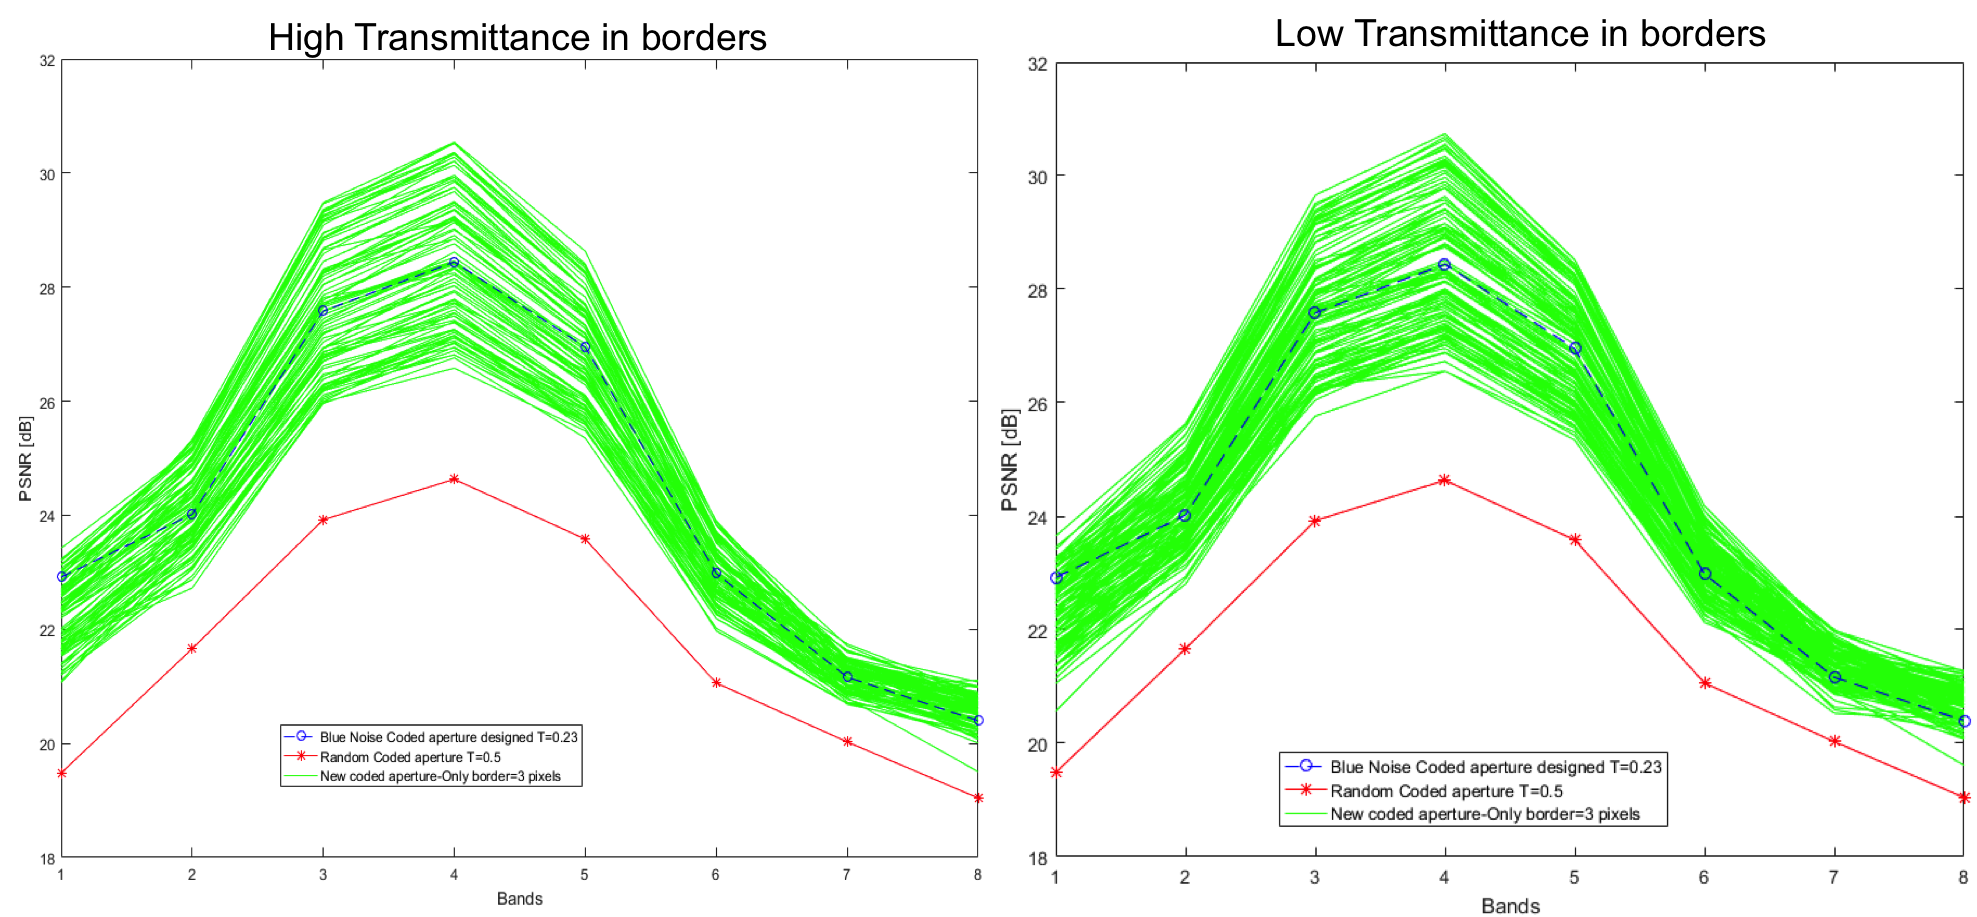
\includegraphics[scale=0.35]{FiguresUpd/simulations.png}
\end{figure}
\end{frame}

%%%%%%%%%%%%%%%%%%%%%%%%%%%%%

\begin{frame}
\frametitle{Experimental results}

\begin{columns}
\column{2in}
\begin{center}
\textbf{Scene}
\begin{figure}
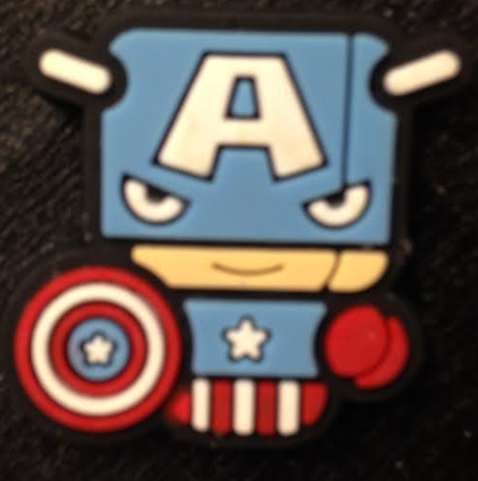
\includegraphics[scale=0.6]{FiguresUpd/real_cel.png}
\end{figure}
\vspace{-10pt}

\end{center}
\column{3in}
\begin{small}
\begin{itemize}
\item Test data cube $\mathcal{F}$: $128 \times 128 \times 10$ 
\item DMD $\Delta_c=13.68\mu m$.
\item A CCD camera $\Delta_d=6.45 \mu m$. 
\item Coded Aperture $T$: $128\times128$ pixels. 
\end{itemize}
\end{small}

\end{columns}
\end{frame}

%%%%%%%%%%%%%%%%%%%%%%%%%%%%%

\begin{frame}
\frametitle{Measurements}

\begin{figure}
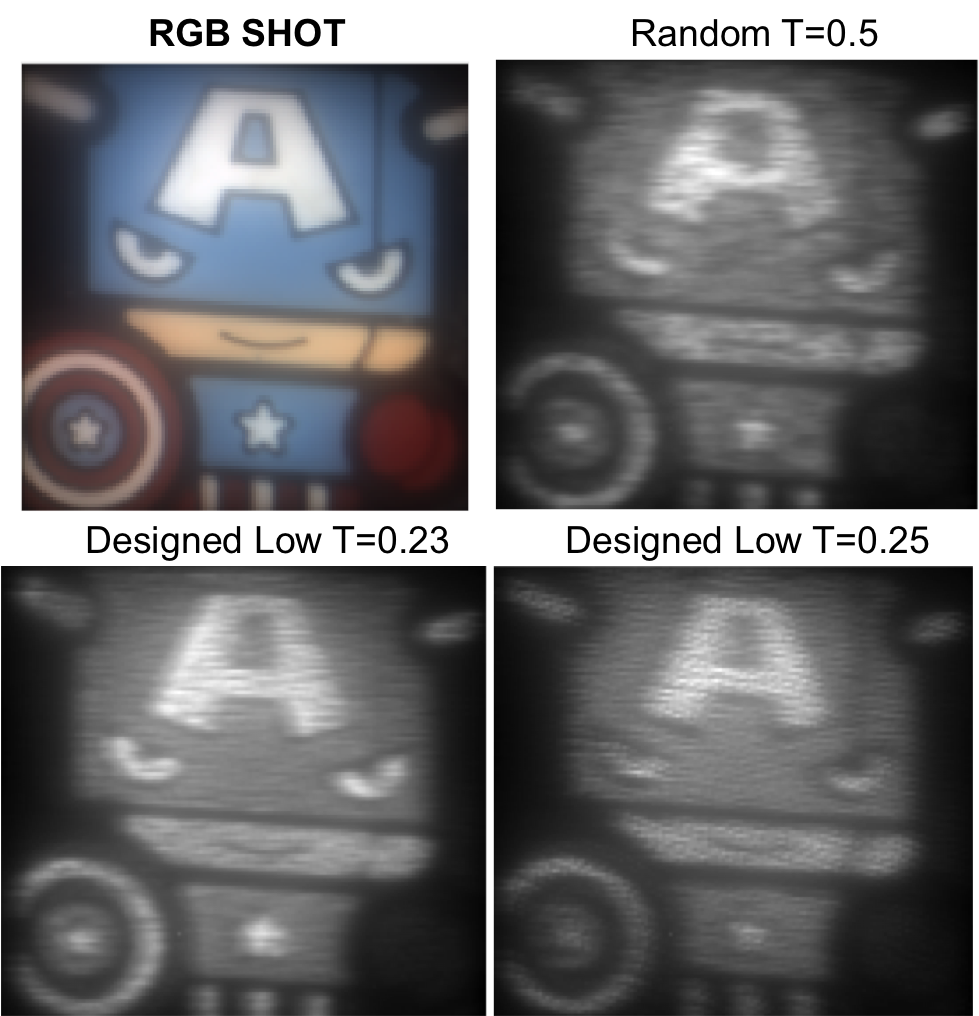
\includegraphics[scale=0.45]{FiguresUpd/meas_all.png}
\end{figure}
\begin{center}
%\begin{scriptsize}
%Original spectral bands
%\end{scriptsize}
\end{center}
\end{frame}


%%%%%%%%%%%%%%%%%%%%%%%%%%%%%

\begin{frame}
\frametitle{Random coded aperture $T=0.5$}

\begin{figure}
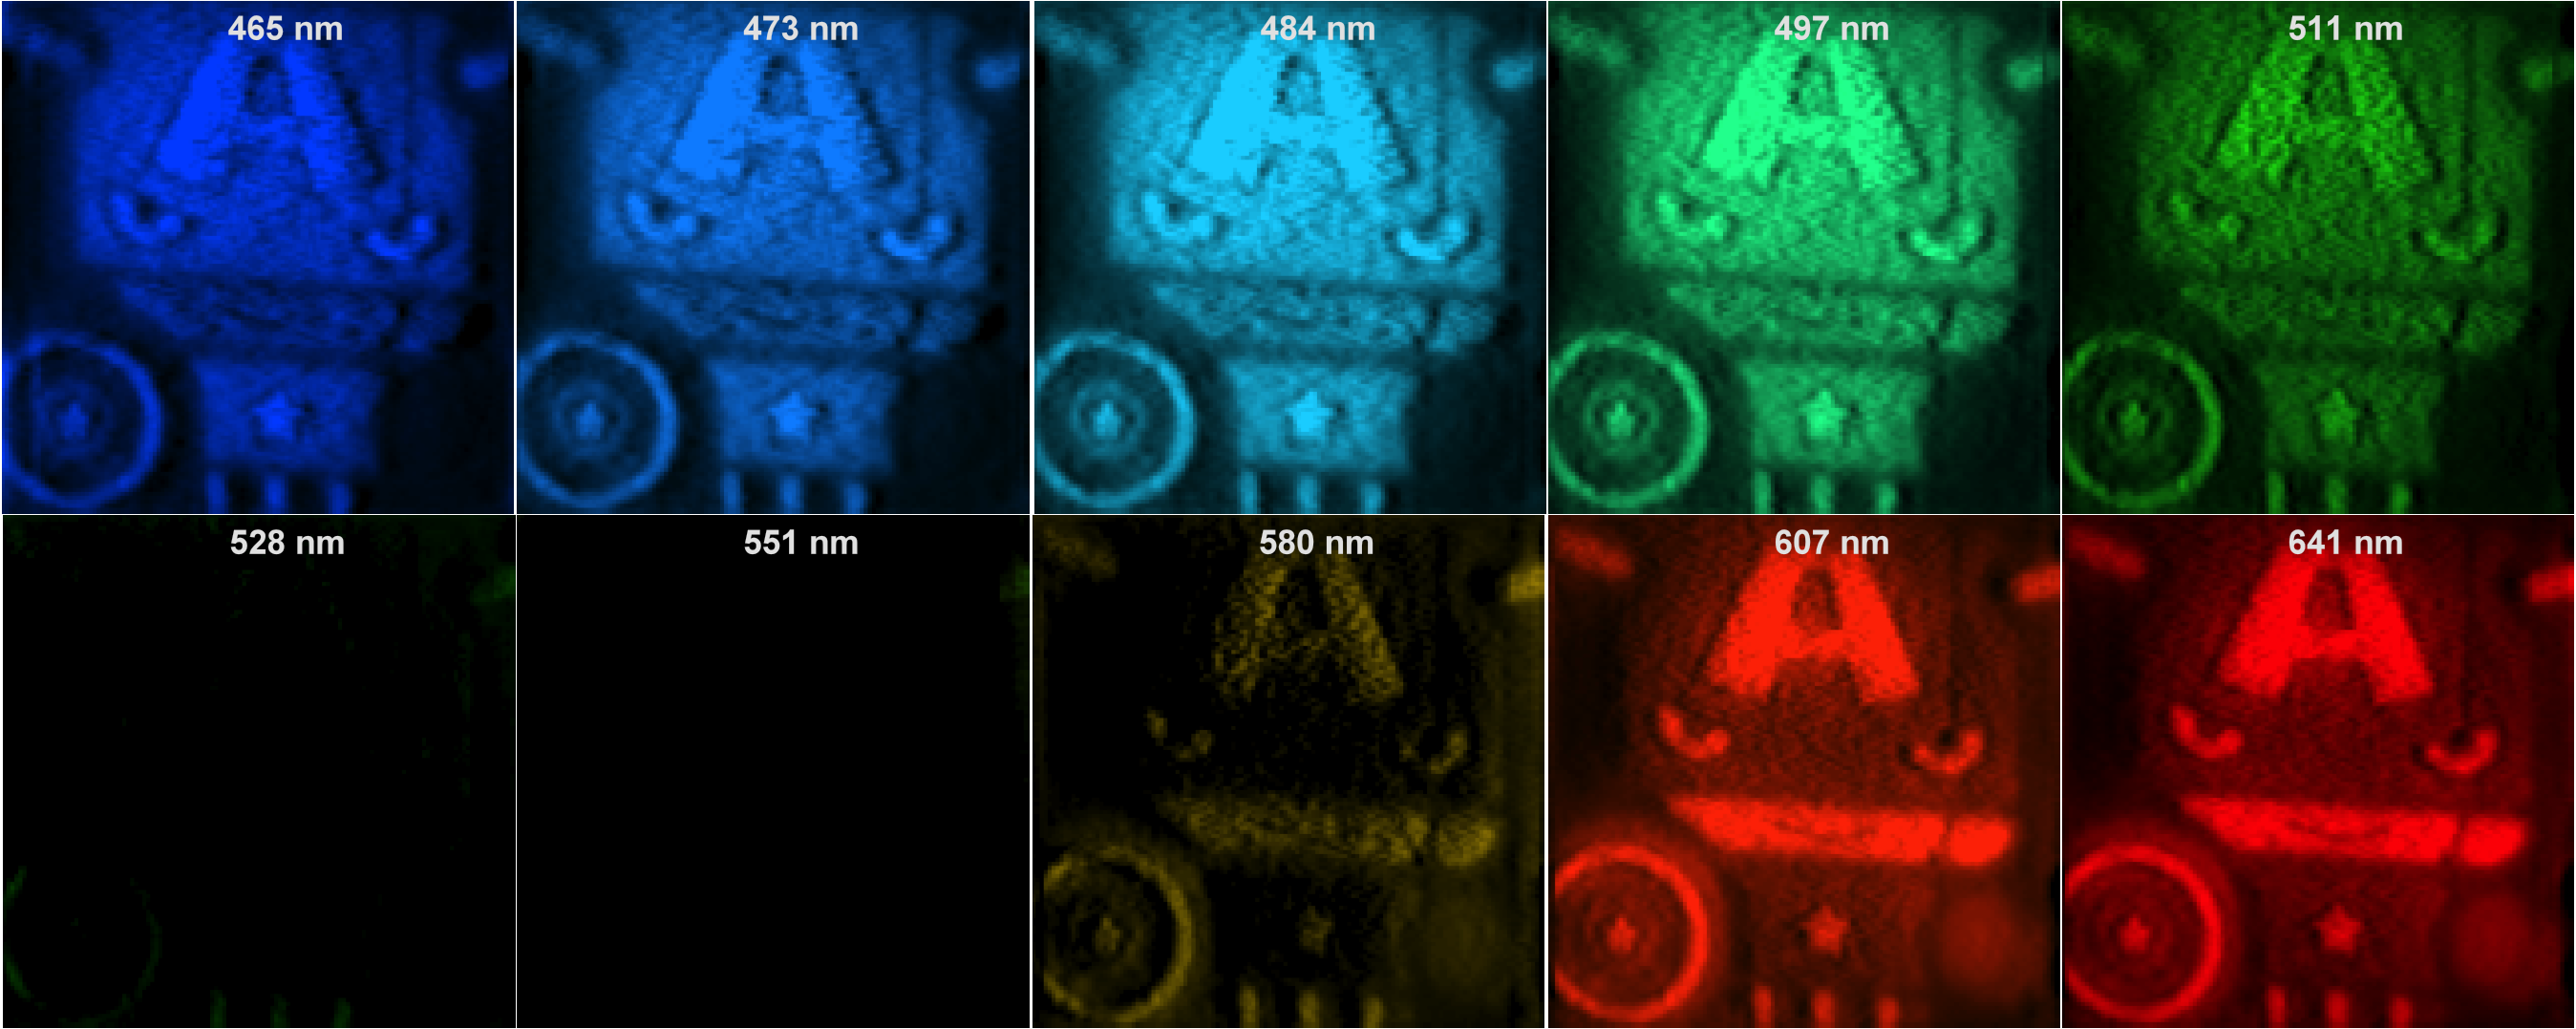
\includegraphics[scale=0.25]{FiguresUpd/real_rand05.png}
\end{figure}
\begin{center}
%\begin{scriptsize}
%Original spectral bands
%\end{scriptsize}
\end{center}
\end{frame}

%%%%%%%%%%%%%%%%%%%%%%%%%%%%%

\begin{frame}
\frametitle{Designed coded aperture, Low T at borders, $T=0.23$}

\begin{figure}
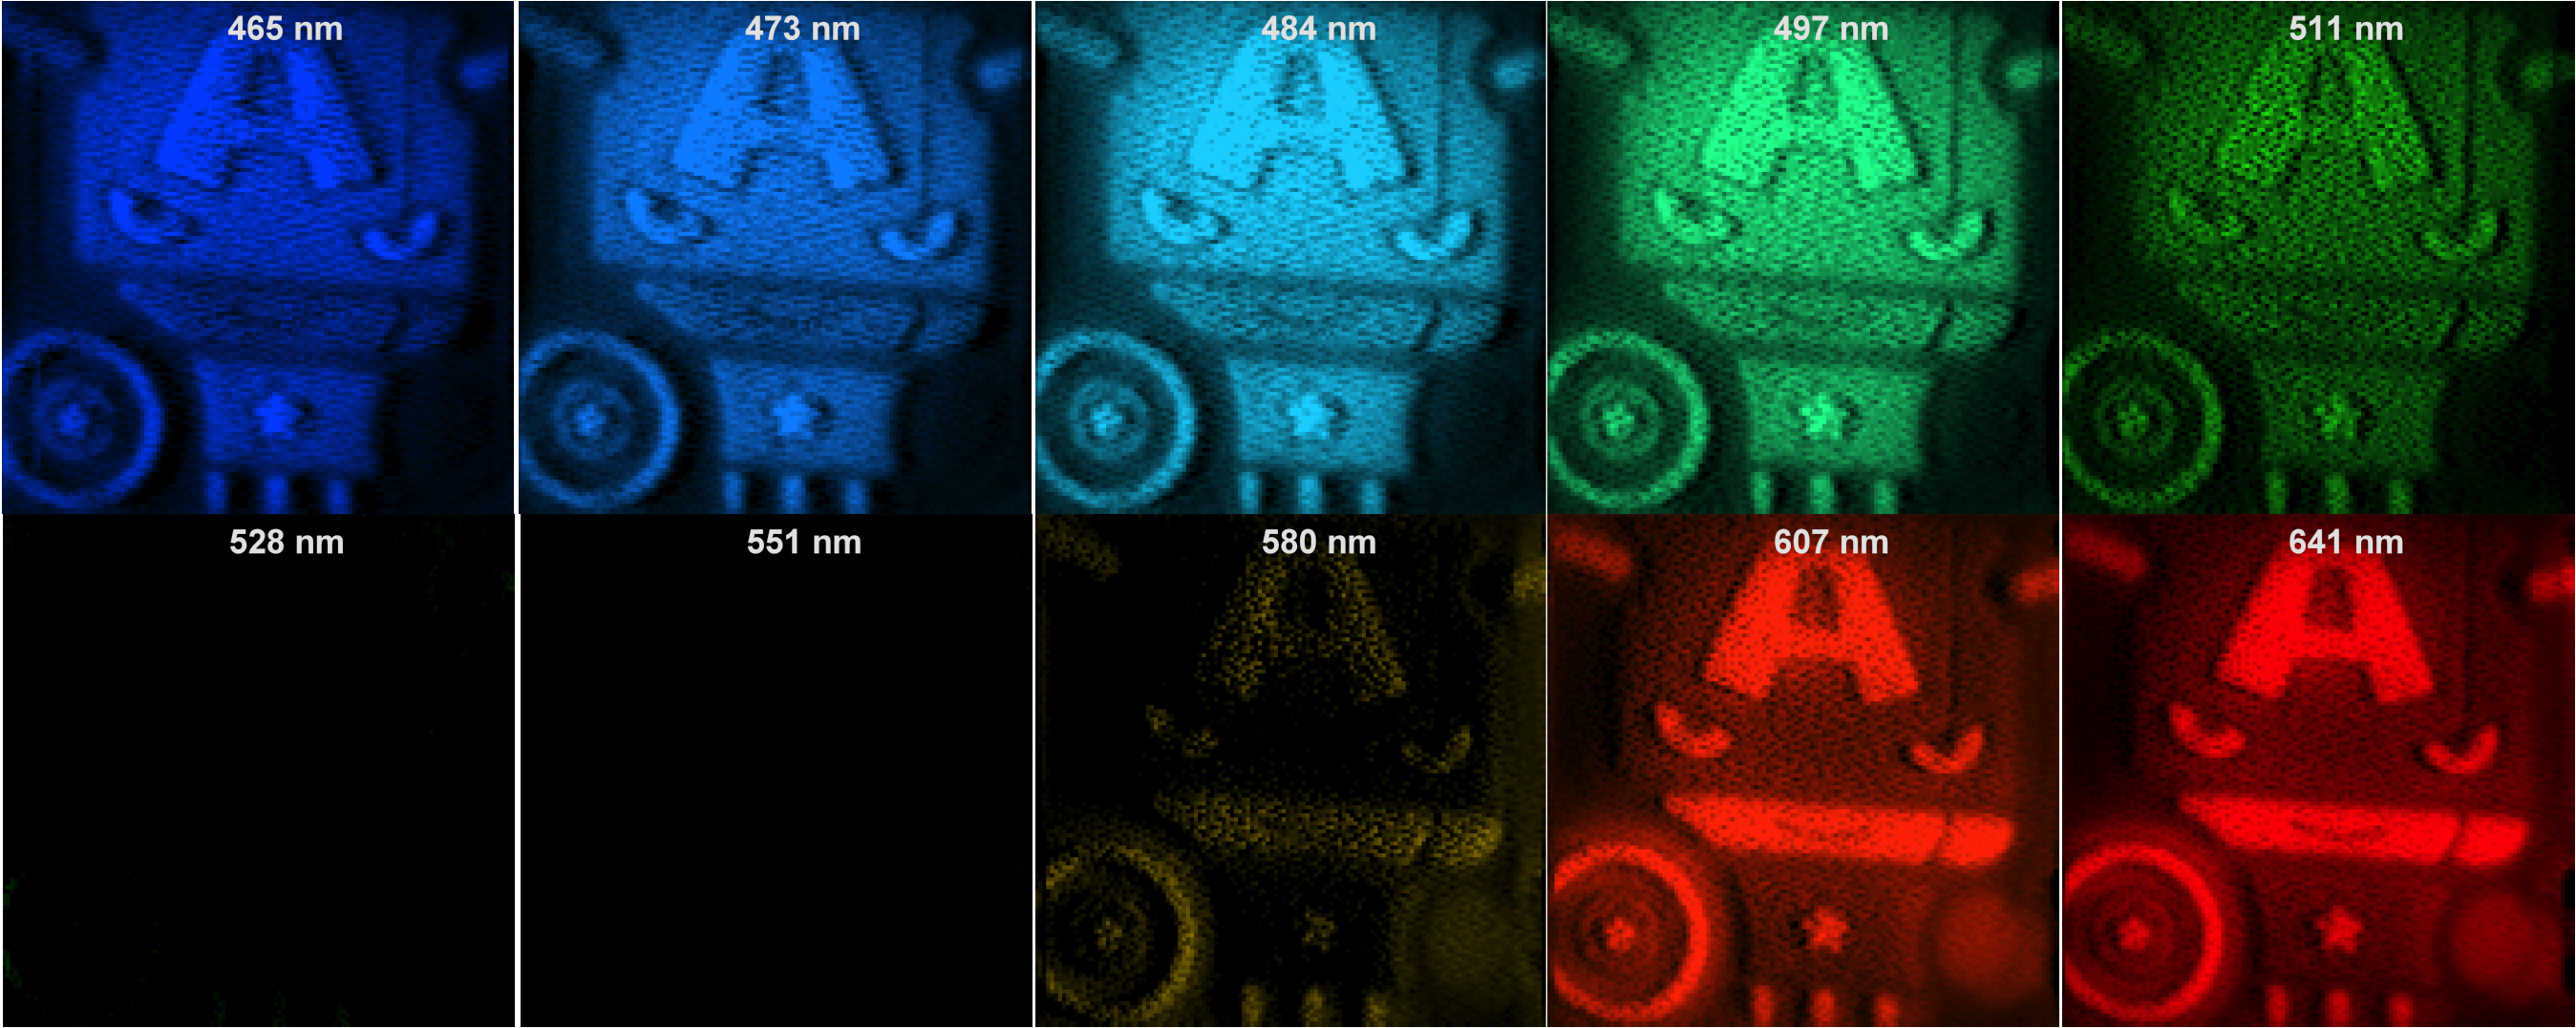
\includegraphics[scale=0.25]{FiguresUpd/real_desig_low.png}
\end{figure}
\begin{center}
%\begin{scriptsize}
%Original spectral bands
%\end{scriptsize}
\end{center}
\end{frame}

%%%%%%%%%%%%%%%%%%%%%%%%%%%%%

\begin{frame}
\frametitle{Designed coded aperture, High T at borders, $T=0.25$}

\begin{figure}
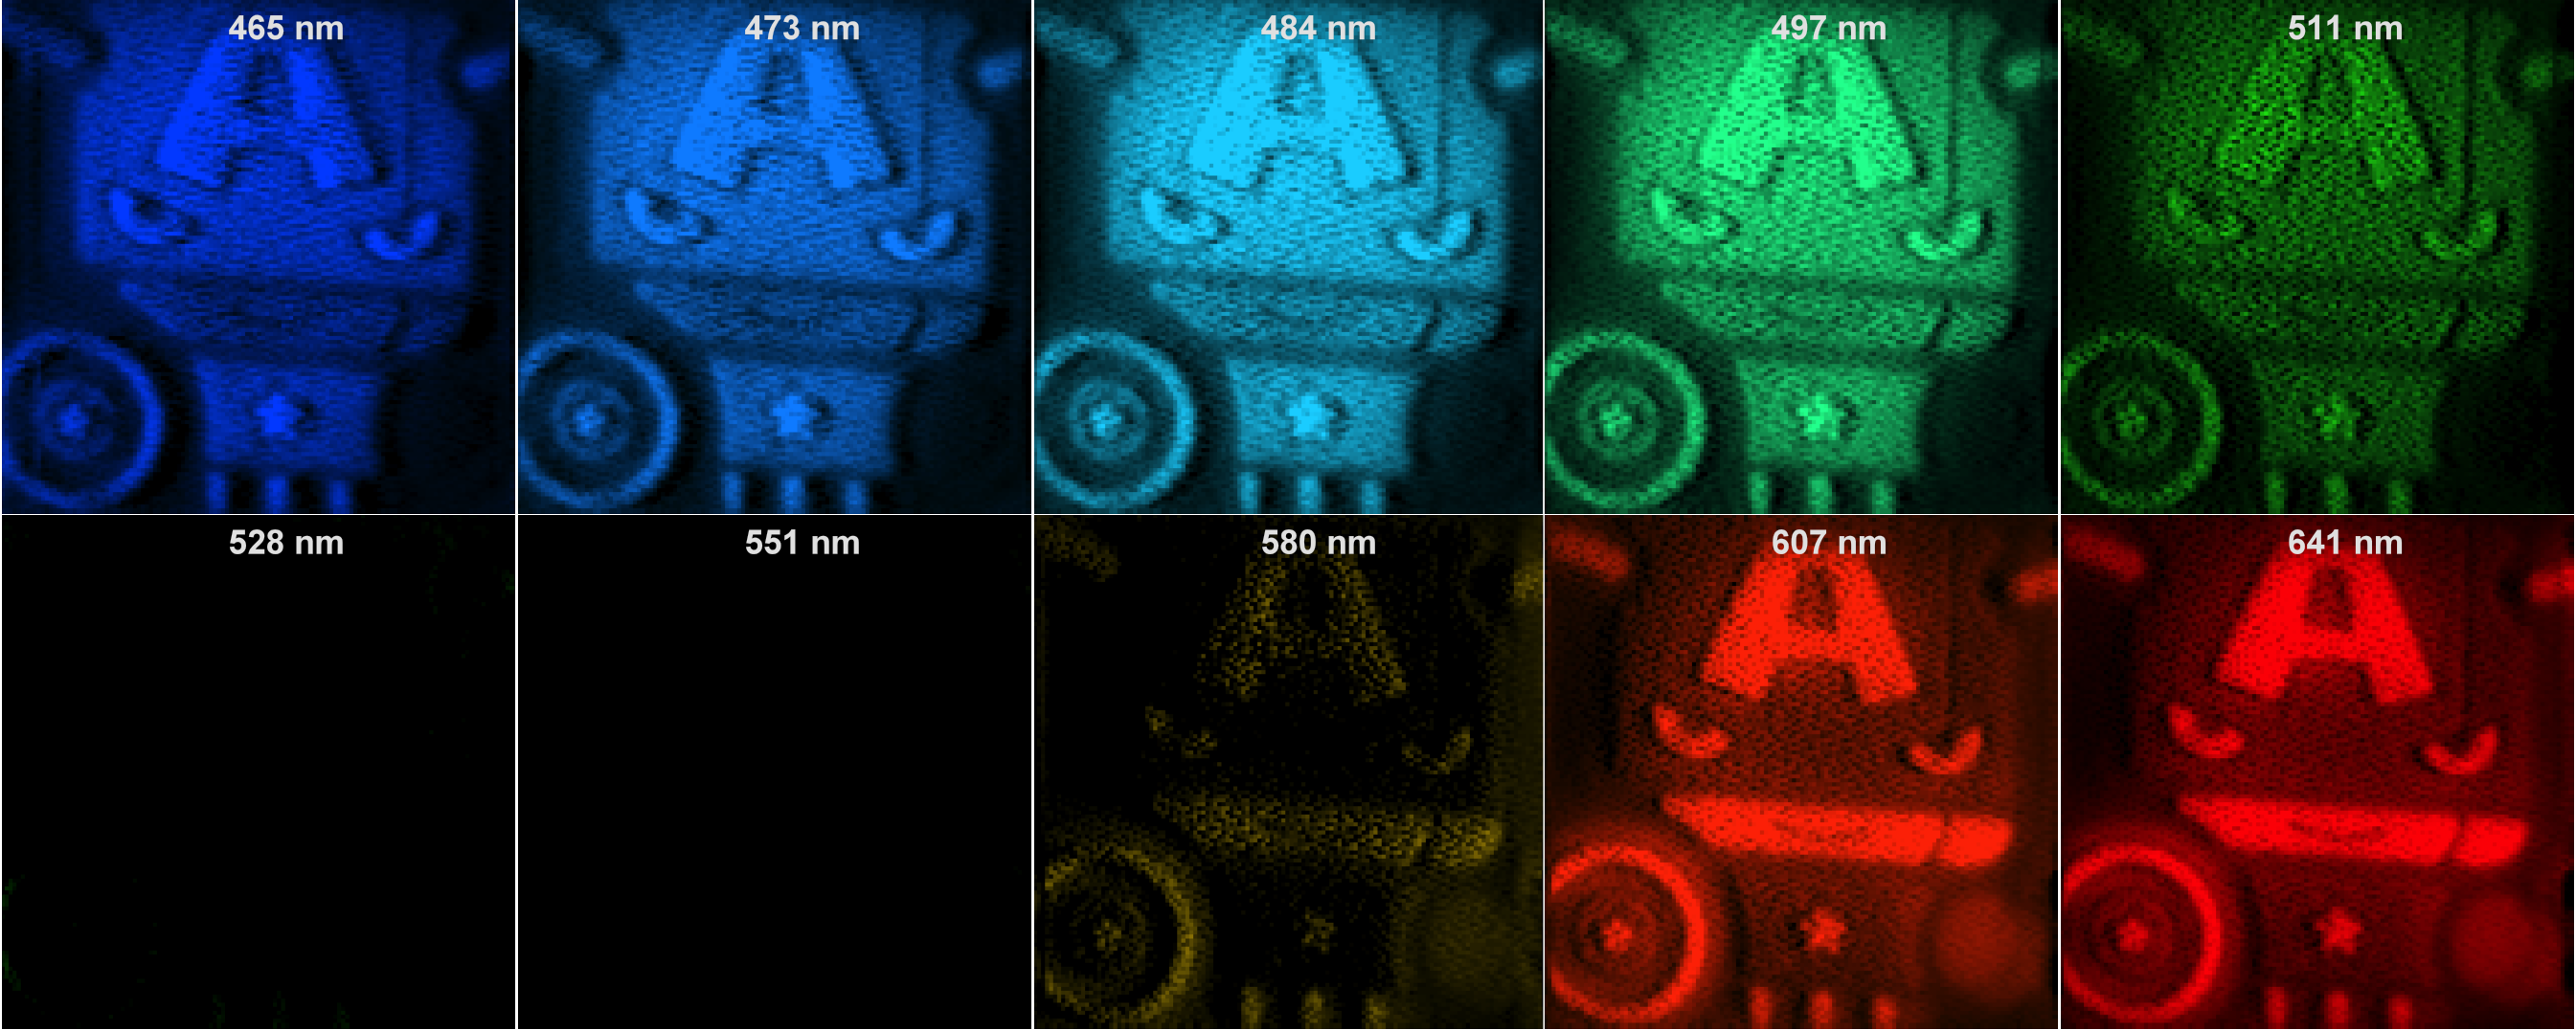
\includegraphics[scale=0.25]{FiguresUpd/real_desig_high.png}
\end{figure}
\begin{center}
%\begin{scriptsize}
%Original spectral bands
%\end{scriptsize}
\end{center}
\end{frame}

%%%%%%%%%%%%%%%%%%%%%%%%%%%%%

\begin{frame}

\begin{figure}
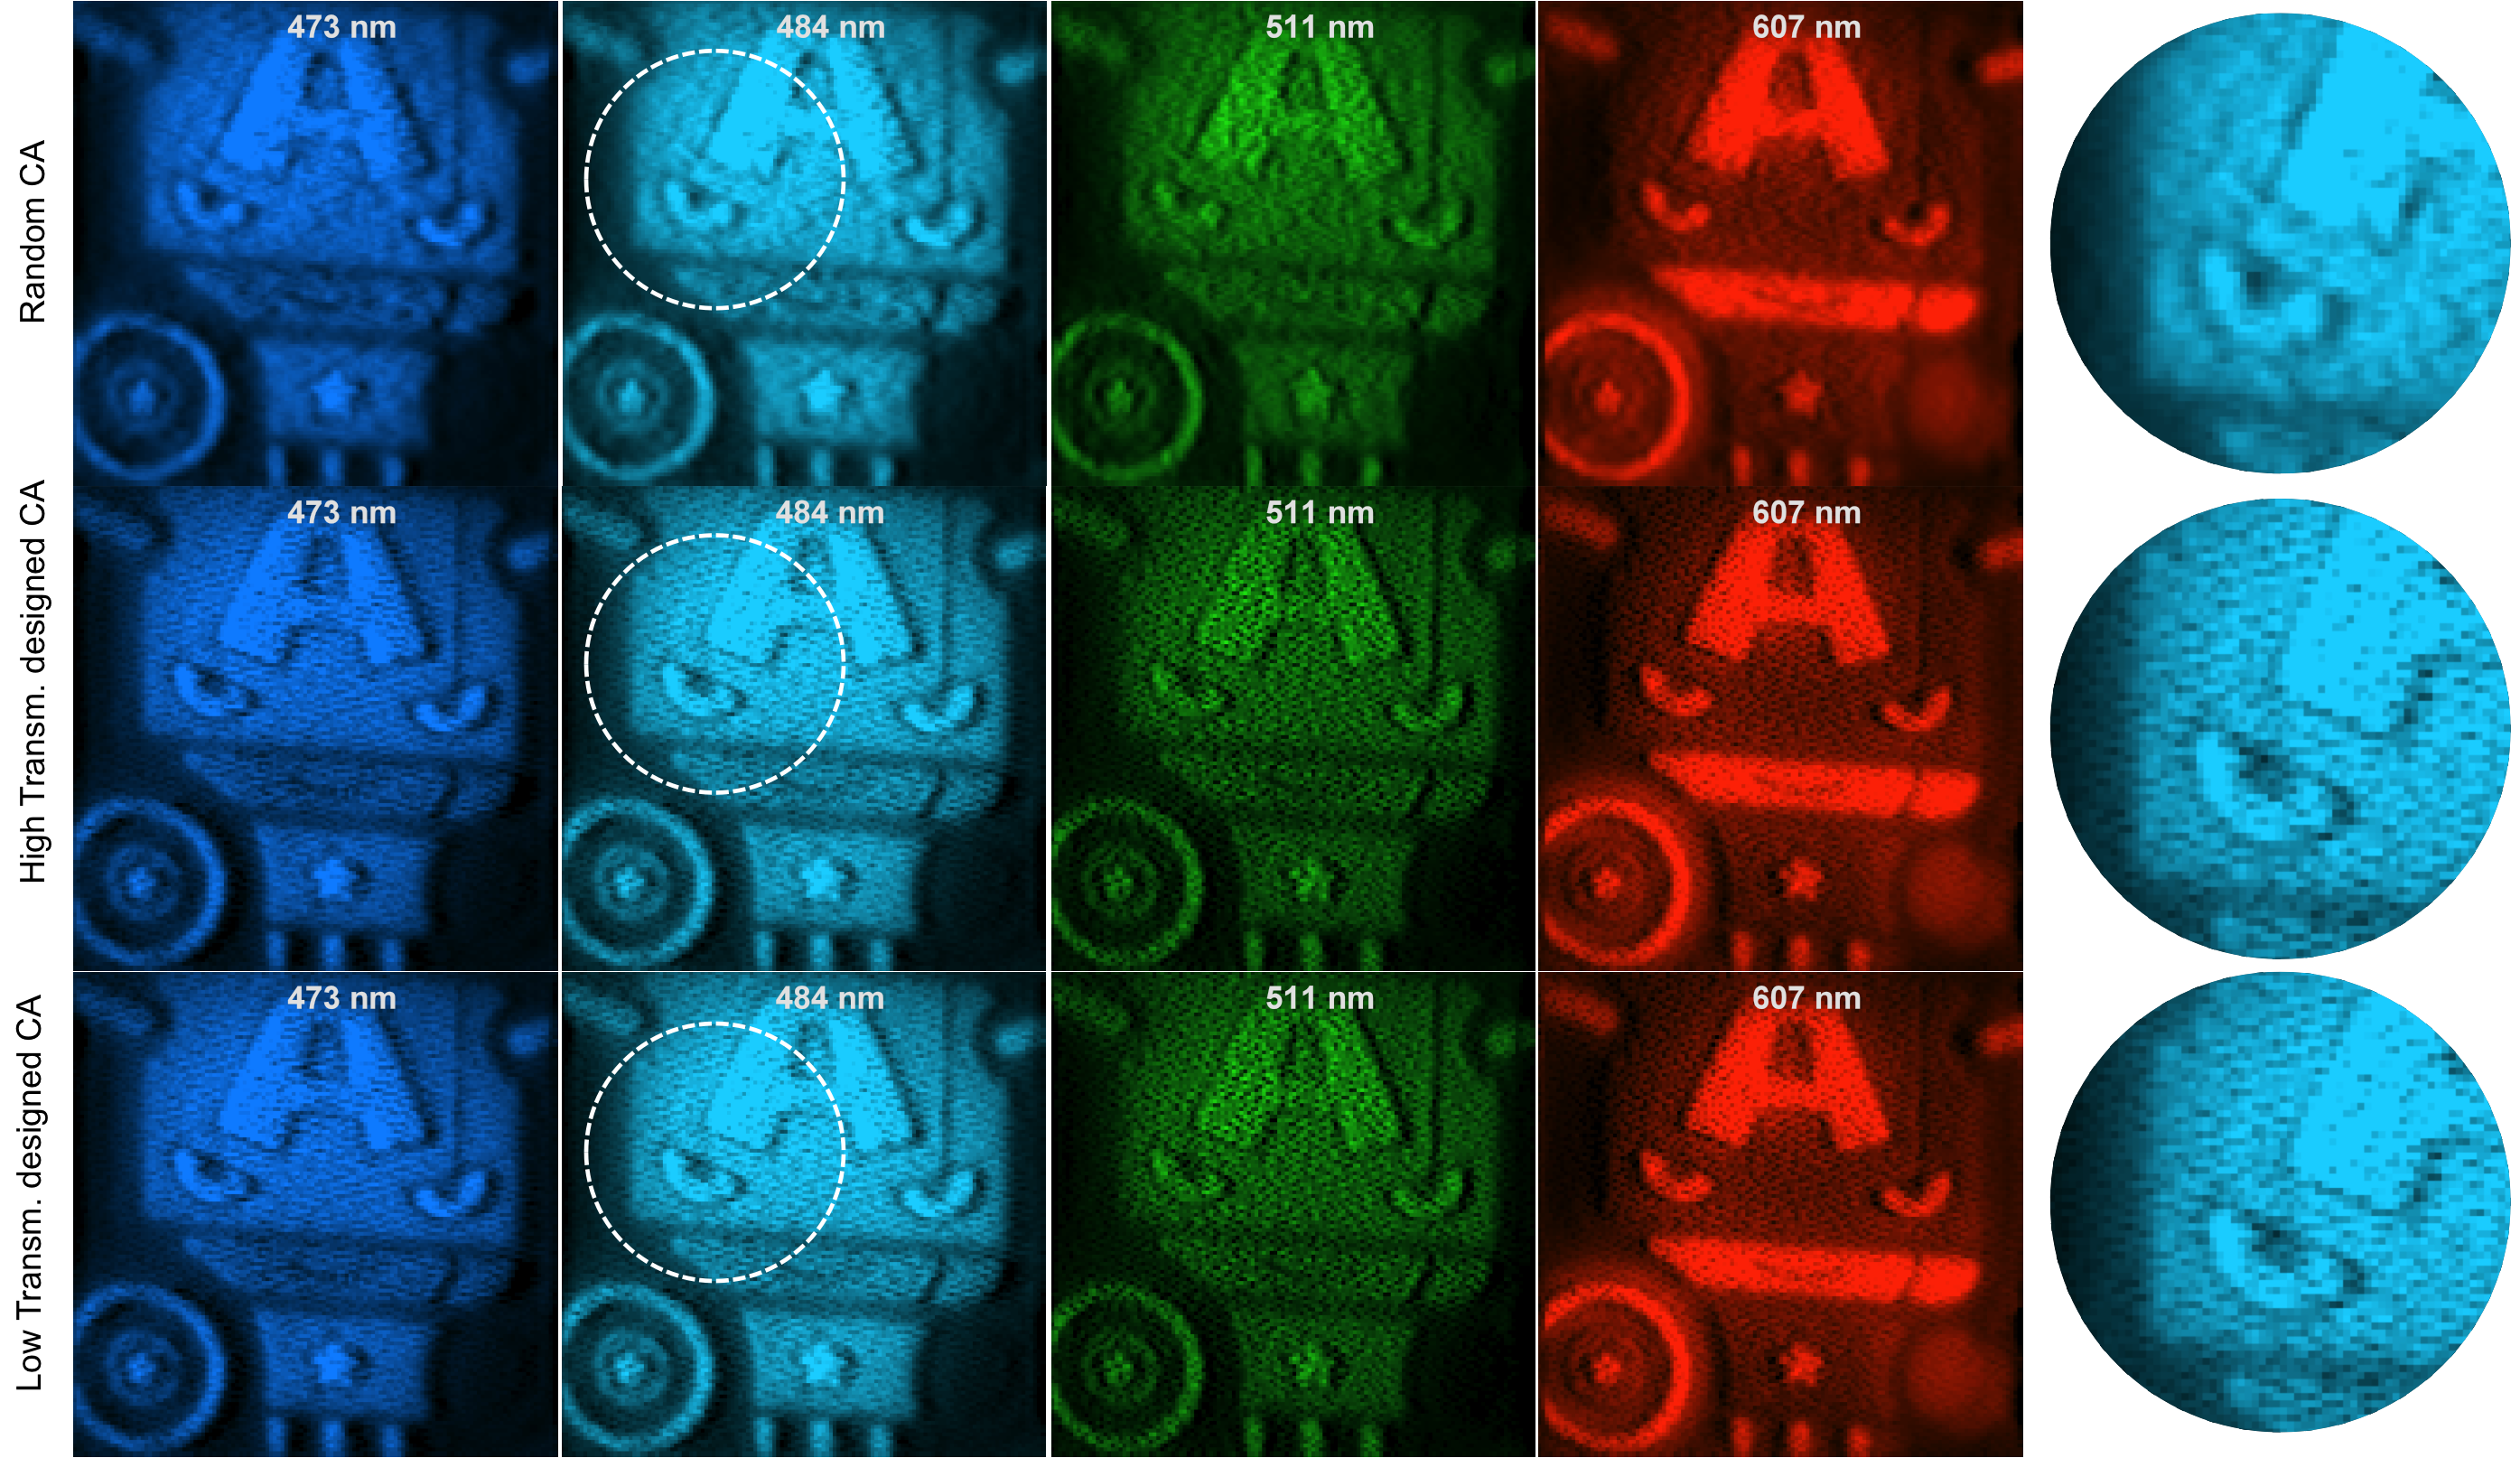
\includegraphics[scale=0.25]{FiguresUpd/real_all.png}
\end{figure}
\begin{center}
%\begin{scriptsize}
%Original spectral bands
%\end{scriptsize}
\end{center}
\end{frame}



%%%%%%%%%%%%%%%%%%%%%%%%%%%%%

%\begin{frame}
%\frametitle{Results: Spatial PSNR}
%
%\begin{scriptsize}
%\hspace{50pt} Transmittance $=0.5$   \hspace{95pt}  Transmittance $=0.25$
%\end{scriptsize}
%\begin{columns}
%\begin{column}{3in}
%\vspace{3pt}
%%\hspace{-15pt}
%%\includegraphics[scale=0.62]{figures/spatialpsnr05nov4.eps}
%\includegraphics[scale=0.42]{figures/05spatial.eps}
%%\hspace{-5pt}
%\end{column}
%
%\begin{column}{4in}
%\hspace{-40pt}
%%\includegraphics[scale=0.63]{figures/spatialpsnr025nov4.eps}
%\includegraphics[scale=0.43]{figures/025spatial.eps}
%\end{column}
%
%\end{columns}
%%\begin{center}
%%\begin{scriptsize}
%%Transmittances of (left) 0.5 and (right) 0.25.
%%\end{scriptsize}
%%\end{center}
%\end{frame}

%%%%%%%%%%%%%%%%%%%%%%%%%%%%%

%\begin{frame}
%\frametitle{Spectral signature reconstruction}
%
%\centering
%\includegraphics[scale=0.34]{FiguresG/bandsignaturessynt4.png}
%
%
%\begin{scriptsize}
%(Up) P1 spectral signature, (Down) P2 spectral signature
%\end{scriptsize}
%
%
%
%\end{frame}

%%%%%%%%%%%%%%%%%%%%%%%%%%%%

\section{Conclusions}
\begin{frame}
\frametitle{Conclusions}

\begin{itemize}
\begin{small}
%\item The use of DMD as a light modulator in CASSI allows multiple advantages over the photomask. However a pixel mismatching problem is included in the system.
\item A forward model of CASSI with side information has been developed. 
\item The model uses the side information for the sensing and the reconstruction process.
%The model avoids creating super-pixels to achieve a pixel-to-pixel correspondence between the pixels of the coded aperture and pixels on the detector. 
\item The coded aperture design exploits key features in the scene such as scene edges.
\item this strategy improves significantly the reconstruction of spectral data cubes, particularly with low SNR measurements.
%The achieved improvement for the reconstruction PSNR is up to $12$ dB, a three fold improvement in spectral resolution and a more accurate signature profile is obtained 
%compared with the CASSI system where super-pixels are created.
\end{small}
\end{itemize}
\end{frame}

%%%%%%%%%%%%%%%%%%%%%%%%%%%%

\begin{frame}
\begin{center}
\textbf{Questions?}\\
\vspace{30pt}
\textbf{Thanks!}
\end{center}


\end{frame}

\end{document}
